%=================================================================
% Droop Control paper — planning / mock-up draft
% Target: MDPI Energies (research article)
%
% PURPOSE OF THIS FILE: This is a structural mock-up to plan the paper and
% organize figures from the modeling/bring-up work. All prose marked with
% "% NOTE" is placeholder argumentation to be rewritten by the author.
% Sections live in sections/*.tex and are \input below.
%=================================================================
\documentclass[energies,article,submit,pdftex,oneauthor]{Definitions/mdpi}

% ---- Extra packages required by the section drafts ----
% mdpi.cls already loads amsmath, graphicx, booktabs, float, adjustbox/changepage.
\usepackage{siunitx}   % \SI, \num, \SIrange used throughout sections 3-5
\usepackage{tabularx}
\newcolumntype{C}{>{\centering\arraybackslash}X} % centered X column for the comparison table

% MDPI internal commands - do not modify
\firstpage{1}
\makeatletter
\setcounter{page}{\@firstpage}
\makeatother
\pubvolume{1}
\issuenum{1}
\articlenumber{0}
\pubyear{2026}
\copyrightyear{2026}
\datereceived{ }
\daterevised{ }
\dateaccepted{ }
\datepublished{ }
\hreflink{https://doi.org/}

% Full title of the paper (Capitalized)
\Title{Controllable Power Sharing in a Hybrid Fuel-Cell/Battery Vehicle Using Droop Control of Off-the-Shelf Boost Regulators with a Robust Outer-Loop Share Controller}
% NOTE: working title — alternatives to consider:
% - "Robust Droop-Based Power Sharing with Commercial Regulator ICs for Hybrid Energy Systems"
% - "A Droop-Injection Architecture for Controllable Power Sharing Using Off-the-Shelf DC-DC Converters"

% MDPI internal command: Title for citation in the left column
\TitleCitation{Controllable Power Sharing Using Droop Control of Off-the-Shelf Boost Regulators}

\newcommand{\orcidauthorA}{0000-0000-0000-000X} % TODO: author ORCID

\Author{Ricky Tang $^{1}$\orcidA{}} % TODO: confirm author list / co-authors (advisor?)
\AuthorNames{Ricky Tang}
\isAPAStyle{%
       \AuthorCitation{Tang, R.}
         }{%
        \isChicagoStyle{%
        \AuthorCitation{Tang, Ricky.}
        }{
        \AuthorCitation{Tang, R.}
        }
}

\address{%
$^{1}$ \quad Affiliation; ricky.tangineering@gmail.com} % TODO: university affiliation

\corres{Correspondence: ricky.tangineering@gmail.com}

% Abstract (Do not insert blank lines, i.e. \\)
\abstract{% NOTE: ~200 words, structured but unheaded. Mock-up:
(1) Background: Multi-source DC power systems (hybrid fuel-cell/battery vehicles, DC microgrids) require controllable power sharing between sources, but custom power-electronics solutions are costly; droop control implemented on commercial regulator ICs offers a low-cost alternative if its accuracy and robustness limitations can be managed.
(2) Methods: We present a droop-injection architecture in which the feedback nodes of two off-the-shelf boost converters (TI TPS61288) are perturbed by multiplying DACs driven from shunt current sense, yielding an electronically commanded droop resistance; an outer power-share loop is closed by a robust $H_\infty$/Youla-parameterized controller synthesized against a 60-corner uncertain plant family.
(3) Results: The synthesized controller achieves $\gamma = 0.686$, exact DC tracking, 11.7~ms delay margin, and worst-corner discrete sensitivity peak of 1.87 versus 26.9 for a nominally tuned PI; an independent 11-state full-order converter model validates the design plant to within 6\% in-band over 432 operating points. Hardware bring-up failures (five converter losses) were diagnosed via parasitic-inductance modeling and ideal-diode soft-start timing analysis, and are shown to be generic multi-converter hazards rather than consequences of the droop architecture.
(4) Conclusions: Droop injection on commercial ICs plus robust outer-loop synthesis provides accurate, tolerance-immune power sharing without custom power stages.}

\keyword{droop control; power sharing; DC microgrid; hybrid vehicle; fuel cell; robust control; $H_\infty$ synthesis; Youla parameterization; boost converter; power path management}

%%%%%%%%%%%%%%%%%%%%%%%%%%%%%%%%%%%%%%%%%%
\begin{document}

% ---------------- Section files ----------------
% ============================================================================
% Section 1 — Introduction + Related Work (mock-up)
% References for the \cite keys live in sections/99_references.tex
% ============================================================================
% PLANNING NOTES — key arguments the author must develop
% ============================================================================
% A1. FRAMING: The scale-vehicle hybrid (fuel cell + battery on a shared DC bus)
%     is a *miniature DC microgrid*. This lets us import the whole droop /
%     current-sharing literature wholesale, and is the justification for
%     submitting to Energies rather than a vehicles venue. Say this explicitly
%     in the first paragraph of the Introduction.
%
% A2. THE GAP (this is the paper's actual novelty — hammer it):
%     Nearly all droop-sharing literature assumes a *custom-designed* converter
%     whose inner current/voltage loop is authored by the researcher (DSP/FPGA
%     PWM generation, full state access). Practical builders of small hybrid
%     systems instead use monolithic, internally-compensated boost ICs
%     (TPS61288 class) where the control loop is inaccessible — the only exposed
%     node is the FB divider. The literature is essentially silent on how to get
%     *commanded, continuously variable* power sharing out of such parts.
%     => Claim: droop realized by MDAC perturbation of the FB node of an
%     off-the-shelf boost IC. Cost/effort of a custom converter avoided;
%     controllability of a centralized scheme retained.
%
% A3. WHY NOT JUST DO IT IN SOFTWARE / COMMUNICATION:
%     Argue that the FC and battery branches are physically separate sources;
%     a comms-based master-slave scheme adds a link, a single point of
%     failure, and latency inside the fast current loop. Droop keeps the fast
%     sharing action analog and local; the slow outer loop only *biases* it.
%     This is the hierarchical-control argument (Guerrero et al.).
%
% A4. WHY ROBUST CONTROL RATHER THAN A PI:
%     The plant seen by the outer share loop is *not* well known: it is the
%     product of (i) IC-internal compensation the vendor only publishes
%     approximately, (ii) INA sense-gain and divider tolerance, (iii) a
%     bus-voltage-dependent and load-current-dependent operating point, and
%     (iv) a droop-injection network with its own attenuation. State the
%     parameter uncertainty box quantitatively (cite the plant model section)
%     and argue this is exactly the setting an H-inf / Youla design addresses,
%     whereas a hand-tuned PI is only valid at one corner.
%     -> Back with the concrete result: worst-corner ||S||_inf 1.87 vs 26.9,
%     all plant corners stable, delay margin ~11.7 ms. MOVE THESE NUMBERS
%     to the Results section but *promise* them in the Introduction.
%
% A5. HONEST LIMITATIONS to pre-empt reviewers (state in Intro, revisit in
%     Discussion): droop trades bus-voltage regulation for sharing accuracy;
%     the MDAC path adds an extra tolerance stack; the approach is bounded by
%     the boost IC's own stability (RHP zero, compensation) so it does not
%     generalize to arbitrary converters without a per-part plant model.
%
% A6. CONTRIBUTION LIST (end of Introduction, 4 bullets — keep parallel):
%     (1) an FB-injection droop mechanism for internally-compensated boost ICs;
%     (2) a small-signal plant model of the two-converter droop-sharing loop
%         including injection attenuation and sense chain, validated against a
%         full-order model;
%     (3) a robust (H-inf/Youla) outer share controller with a documented
%         synthesis and gate-check procedure;
%     (4) experimental validation on a scale fuel-cell/battery vehicle.
%
% A7. TODO(author): decide whether to cite the scale-vehicle / RC-testbed
%     literature at all. If a suitable "hardware-in-the-loop scale testbed"
%     reference exists, add it to justify scale validation as scientifically
%     meaningful. Currently no such citation is included.
%
% A8. TODO(verify): every \bibitem in 99_references.tex was checked to exist
%     and carries a DOI or stable URL, but several carry % TODO(verify) marks
%     for author list / volume — re-check against Crossref before submission;
%     MDPI copy-edits references against Crossref.
% ============================================================================

\section{Introduction}
\label{sec:intro}

% NOTE: Paragraph 1 should establish the application context and assert the
% microgrid framing (A1). Keep it short; do not oversell hydrogen.
Hybridizing a fuel cell with a battery is the standard remedy for the fuel
cell's poor transient response and its intolerance of load steps and reverse
current. In such a powertrain both sources feed a common DC link through
dedicated converters, and the question of how instantaneous load current is
apportioned between them becomes a control problem in its own right. Structurally
this is the same problem studied under the heading of DC microgrids, where
multiple dissimilar sources share a bus through parallel-connected
converters~\cite{dragicevic2016part1,dragicevic2016part2,gao2018primary}.

% NOTE: Paragraph 2 introduces droop as the incumbent decentralized answer and
% states its two well-known weaknesses (voltage deviation, sharing error under
% line/parameter mismatch). This sets up why an outer loop is needed at all.
The conventional answer is droop control: each converter deliberately reduces
its output voltage in proportion to its output current, so that a virtual output
resistance sets the sharing ratio without any communication between
units~\cite{guerrero2011hierarchical,tah2016adaptive}. Droop is attractive because
it is local, fast and inherently redundant, but it is well documented that it
trades bus-voltage regulation against sharing accuracy, and that mismatched line
and converter parameters corrupt the achieved split~\cite{anand2013distributed,lu2014adaptive}.
A large body of work therefore adds a secondary or distributed layer that trims
the droop coefficients or the voltage
references~\cite{nasirian2015cooperative,tucci2018plugandplay,kumar2020distributed}.

% NOTE: Paragraph 3 is the pivot — the hardware-realization gap (A2). This is
% the paragraph the whole paper hangs on. Author should be blunt: existing
% droop work presumes a converter you designed yourself.
Almost without exception, that literature presumes a converter whose inner loop
the designer owns: modulation is generated in a DSP or FPGA, and the droop term
is simply added to a software voltage reference. Practitioners building small
hybrid systems rarely enjoy that freedom. Power stages are increasingly bought as
monolithic, internally-compensated regulator ICs, in which the control loop is
sealed and the only user-accessible node is the feedback divider. For such parts
the standard droop recipe has no point of entry, and designers fall back on
fixed resistive droop, on a hard master--slave split, or on abandoning
controllable sharing altogether.

% NOTE: Paragraph 4 states the proposed mechanism concretely. Do NOT get into
% circuit values here — forward-reference the hardware section.
This paper shows that controllable droop can nevertheless be obtained from such
a device. A multiplying digital-to-analogue converter (MDAC) injects a
current-proportional perturbation into the feedback node of each off-the-shelf
boost regulator, synthesizing a commanded, continuously variable output
resistance in analogue hardware. The fast sharing action remains local to each
converter; a slow digital outer loop merely commands the droop ratio, and hence
the steady-state power split, between the fuel-cell and battery branches.

% NOTE: Paragraph 5 motivates the robust outer controller (A4). Emphasize
% *why the plant is uncertain*, not just that robust control is fashionable.
Because the resulting plant is assembled from an IC whose internal compensation
is only approximately published, a sense amplifier and divider network with
finite tolerance, and an operating point that moves with bus voltage and load,
its parameters are known only within a box rather than exactly. This is precisely
the setting for robust synthesis, and $\mathcal{H}_\infty$ and related methods
have already been applied to microgrid voltage and sharing
loops~\cite{sedhom2019hinf,hosseinzadeh2024robust,mirjafari2022robust}. We
accordingly design the outer share controller by $\mathcal{H}_\infty$/Youla
synthesis over the parameter corners rather than by tuning a PI at nominal.

% NOTE: Paragraph 6 = contributions. Use A6. Keep the four items parallel.
The contributions of this work are: (i) a feedback-injection droop mechanism
that gives commanded power sharing from internally-compensated, off-the-shelf
boost regulators; (ii) a small-signal model of the two-converter droop-sharing
loop that accounts for the injection attenuation and the current-sense chain,
validated against an independently constructed full-order model; (iii) a robust
outer share controller with a documented synthesis and verification procedure;
and (iv) experimental validation on a scale fuel-cell/battery vehicle.

% NOTE: Paragraph 7 = roadmap. Author fills in once section numbering is final.
The remainder of the paper is organized as follows. Section~\ref{sec:related}
reviews power-sharing methods and positions the proposed approach.
Section~\ref{sec:droop} develops the droop design and gain selection;
Section~\ref{sec:robust} the robust share controller; Section~\ref{sec:board-design}
the board and power-path hardware; Section~\ref{sec:bringup} the bring-up
diagnosis; Section~\ref{sec:mimo} the MIMO outlook.

\section{Related Work}
\label{sec:related}

\subsection{Droop Control and Its Refinements}

% NOTE: Establish the canonical V-I droop / virtual resistance formulation and
% its known limits. Cite the two survey papers so a reviewer sees breadth.
Conventional voltage--current droop emulates a series resistance $R_d$ at each
converter output, so that $v_o = V^\ast - R_d i_o$. Sharing accuracy improves
with larger $R_d$ while bus regulation degrades, a tension that is the
starting point of most subsequent work~\cite{dragicevic2016part1,gao2018primary}.
Virtual-resistance implementations move this behaviour into the controller rather
than dissipating it, and adaptive schemes vary $R_d$ online according to
converter rating, state of charge or measured sharing
error~\cite{tah2016adaptive,lu2014adaptive,khorsandi2024adaptive}.

% NOTE: Second paragraph should cover the secondary/distributed correction
% layer, and make the point that these schemes reintroduce communication —
% which is the wedge for our comparison table.
Because purely local droop cannot remove the steady-state voltage deviation, a
secondary layer is usually added. Distributed and consensus-based schemes
exchange voltage and current estimates over a sparse communication graph to
restore the bus and equalize per-unit currents
simultaneously~\cite{nasirian2015cooperative,anand2013distributed,kumar2020distributed},
and plug-and-play designs provide stability guarantees that are independent of
the network topology~\cite{tucci2018plugandplay}. These methods achieve excellent
accuracy at the cost of a communication link and its associated latency and
failure modes.

\subsection{Alternatives to Droop}

% NOTE: This subsection must be genuinely fair to the alternatives — reviewers
% punish strawmanning. Cover master-slave, average current sharing, DC bus
% signaling, MPC. Each gets one or two sentences plus a citation.
Active current-sharing methods predate the microgrid framing. Master--slave and
average-current-sharing architectures for paralleled supply modules were
classified early and remain the industrial default where the modules are
identical and co-located~\cite{luo1999classification,panov2008stability}. They
give near-exact sharing but require a dedicated share bus and degrade poorly
when the master fails.

DC bus signaling dispenses with an explicit link by encoding mode transitions in
the bus voltage itself, so that each unit infers the system state
locally~\cite{schonberger2006dbs,panda2021dbs}. The method is elegant for
coarse mode arbitration but does not deliver a continuously commandable split.

Optimization-based supervision, particularly model predictive control, has been
applied extensively to fuel-cell hybrid powertrains to schedule the source split
against fuel economy and degradation
objectives~\cite{vermillion2011mpc,hu2021mpcreview,zhou2022mpc}. Such strategies
operate above the converter loops: they decide \emph{what} the split should be, and
still require an actuation mechanism to enforce it. The present work is
complementary rather than competing, and in fact supplies exactly that
mechanism.

\subsection{Power Sharing in Fuel-Cell Hybrid Vehicles}

% NOTE: Ground the work in the FC/battery application; make the frequency-
% separation argument (FC slow, battery fast) since it explains why the share
% setpoint is slow-moving and why a slow robust outer loop suffices.
In fuel-cell hybrids the split is not arbitrary: the stack must be protected
from fast transients, which are absorbed by the battery or a supercapacitor,
while the stack carries the slow-moving mean
demand~\cite{thounthong2007control,garcia2016statemachine,li2022dcbusregulation}.
This frequency separation is usually enforced by filtering the demand signal or
by a rule-based supervisor. Droop achieves the same separation as a structural
property when the branches are given different output impedances, which is one
reason droop-based energy management has been reported for fuel-cell
tramways and hybrid buses~\cite{garcia2016statemachine,li2022dcbusregulation}.

\subsection{Robust Control of Sharing Loops}

% NOTE: Short subsection. Point is: robust methods exist for microgrid loops but
% are applied to custom converters with accessible states; nobody applies them
% to a droop loop whose actuator is an MDAC on a commercial IC's FB pin.
Robust synthesis has been used to certify microgrid loops against parameter
drift, constant-power-load negative impedance and communication
delay~\cite{sedhom2019hinf,hosseinzadeh2024robust,mirjafari2022robust}. These
results confirm the value of a worst-case formulation, but they are invariably
applied to converters whose internal dynamics are designed alongside the
controller. Applying the same discipline to a loop whose actuator is an MDAC
perturbing the feedback pin of a commercial regulator, and whose plant gain
therefore inherits vendor tolerances, appears not to have been reported.

\subsection{Positioning}

% NOTE: Refer to the table explicitly and state the one-line thesis of the paper.
Table~\ref{tab:comparison} summarizes the trade-offs. The proposed approach
occupies a cell that the existing methods do not: it retains the commandability
of a centralized scheme and the robustness of a droop scheme, while requiring
neither a custom power stage nor a communication link inside the fast loop.

% ---------------------------------------------------------------------------
% Comparison table
% ---------------------------------------------------------------------------
\begin{table}[H]
\caption{Comparison of DC power-sharing methods against the criteria relevant to
a low-cost hybrid powertrain. Ratings are qualitative:
\textbullet\textbullet\textbullet{} = favourable,
\textbullet{} = unfavourable.}
\label{tab:comparison}
\newcommand{\rgood}{\textbullet\textbullet\textbullet}
\newcommand{\rmid}{\textbullet\textbullet}
\newcommand{\rbad}{\textbullet}
\begin{adjustwidth}{-\extralength}{0cm}
\begin{tabularx}{\fulllength}{lCCCCCl}
\toprule
\textbf{Method} & \textbf{Hardware} & \textbf{Comms} & \textbf{Split} &
\textbf{Robustness to} & \textbf{Off-the-shelf} & \textbf{Refs} \\
 & \textbf{cost} & \textbf{required} & \textbf{controllability} &
\textbf{converter tol.} & \textbf{ICs usable} & \\
\midrule
Fixed resistive droop        & \rgood & none    & \rbad  & \rbad  & \rgood & \cite{dragicevic2016part1,gao2018primary} \\
Virtual-resistance droop     & \rmid  & none    & \rmid  & \rmid  & \rbad  & \cite{tah2016adaptive,lu2014adaptive} \\
Adaptive / consensus droop   & \rmid  & sparse  & \rgood & \rgood & \rbad  & \cite{nasirian2015cooperative,anand2013distributed,kumar2020distributed} \\
Master--slave current share  & \rbad  & share bus & \rgood & \rmid & \rbad  & \cite{luo1999classification} \\
Average current sharing      & \rbad  & share bus & \rmid & \rmid  & \rbad  & \cite{luo1999classification,panov2008stability} \\
DC bus signaling             & \rgood & none    & \rbad  & \rmid  & \rmid  & \cite{schonberger2006dbs,panda2021dbs} \\
Supervisory MPC / EMS        & \rmid  & to supervisor & \rgood & n/a $^{a}$ & n/a $^{a}$ & \cite{vermillion2011mpc,hu2021mpcreview,zhou2022mpc} \\
\midrule
\textbf{This work:} MDAC feedback-injection droop
                             & \rgood & none $^{b}$ & \rgood & \rgood $^{c}$ & \rgood & --- \\
\bottomrule
\end{tabularx}
\end{adjustwidth}
\noindent{\footnotesize
$^{a}$ Supervisory strategies presuppose an underlying actuation mechanism and
are therefore complementary to, not substitutes for, the rows above.
$^{b}$ No communication inside the fast sharing loop; a low-rate link carries
only the share setpoint.
$^{c}$ By construction of the robust outer controller over the parameter
corners; see Section~\ref{sec:robust}.}
\end{table}

% NOTE(author): the table uses MDPI's adjustwidth/tabularx macros from the
% Energies class (\fulllength, \extralength, column type C). The agent draft
% used threeparttable-style \tablenotes, which the MDPI class does NOT load —
% replaced here with plain footnote markers. Verify column type C compiles;
% if not, define \newcolumntype{C}{>{\centering\arraybackslash}X}.
        % Introduction + related work + method comparison table
% =====================================================================
% SECTION: Droop Control Design and Gain Selection
% Sources of truth:
%   controller_design/system_model.md  (§2, §3, §4, §8)
%   teensy_controller/teensy_controller.ino  (lines 451-468, 2180-2190, 2760-2840)
%   CLAUDE.md §5, §7, addendum 2026-07-10 and 2026-07-11
% =====================================================================
\section{Droop Control Design and Gain Selection}
\label{sec:droop}

\subsection{Design Ethos: Power Sharing Without a Custom Power Stage}
\label{sec:droop:ethos}

% NOTE(author): rewrite this paragraph in the paper's voice; the argument is right
% but the prose is engineer-terse. Emphasise the "commodity silicon + analog
% perturbation" framing, which is the paper's actual contribution claim.
The power-sharing objective for a hybrid fuel-cell/battery vehicle is to place a commanded
fraction $\alpha_{req}$ of the bus current on the fuel cell and the remainder on the
battery, continuously and under load transients. The conventional route is a
purpose-designed dual-input converter with a shared, digitally arbitrated current loop.
This work deliberately takes the opposite route: both sources are boosted by
\emph{unmodified, off-the-shelf} converters (Texas Instruments TPS61288, constant-off-time
peak-current-mode boost), and sharing is imposed by \emph{perturbing each regulator's
feedback node} with a signal proportional to that regulator's own output current. Each
converter therefore behaves as a Th\'evenin source with an electronically programmable
output resistance, and the two sources share current by classical droop --- but with a
droop coefficient the microcontroller can rewrite at any instant.

The advantages that motivate this choice are practical rather than theoretical:

\begin{enumerate}
  \item \textbf{No custom power stage.} The converters keep their datasheet compensation,
        protection, soft-start, and thermal behaviour. Nothing in the high-current path is
        bespoke, so the failure modes are the vendor's characterised ones.
  \item \textbf{The fast loop stays analog.} Current sensing, scaling, and injection are
        continuous-time hardware; the digital controller only \emph{trims a coefficient}.
        Sharing does not collapse if the MCU is late, and the loop is not sampled at the
        converter's switching time scale.
  \item \textbf{Graceful degradation.} With the digital-to-analog converters parked at a
        fixed code the board is still a working, statically drooped parallel supply. The
        control law is an enhancement, not a prerequisite for operation.
\end{enumerate}

The per-channel signal chain that realises this is fixed by the board and is shown in
Figure~\ref{fig:droop-chain}: the channel's output current is measured by an INA253A1
integrated shunt amplifier, scaled by a 12-bit AD5443 multiplying DAC (MDAC) operating in
voltage-switching mode, buffered and amplified by an OPA197, and injected through a
resistor into the boost converter's feedback divider node.

\begin{figure}[H]
  \centering
  % FIGURE FILE: controller_design/figures/droop_signal_chain.svg
  % (convert to PDF for LaTeX: inkscape --export-type=pdf droop_signal_chain.svg)
  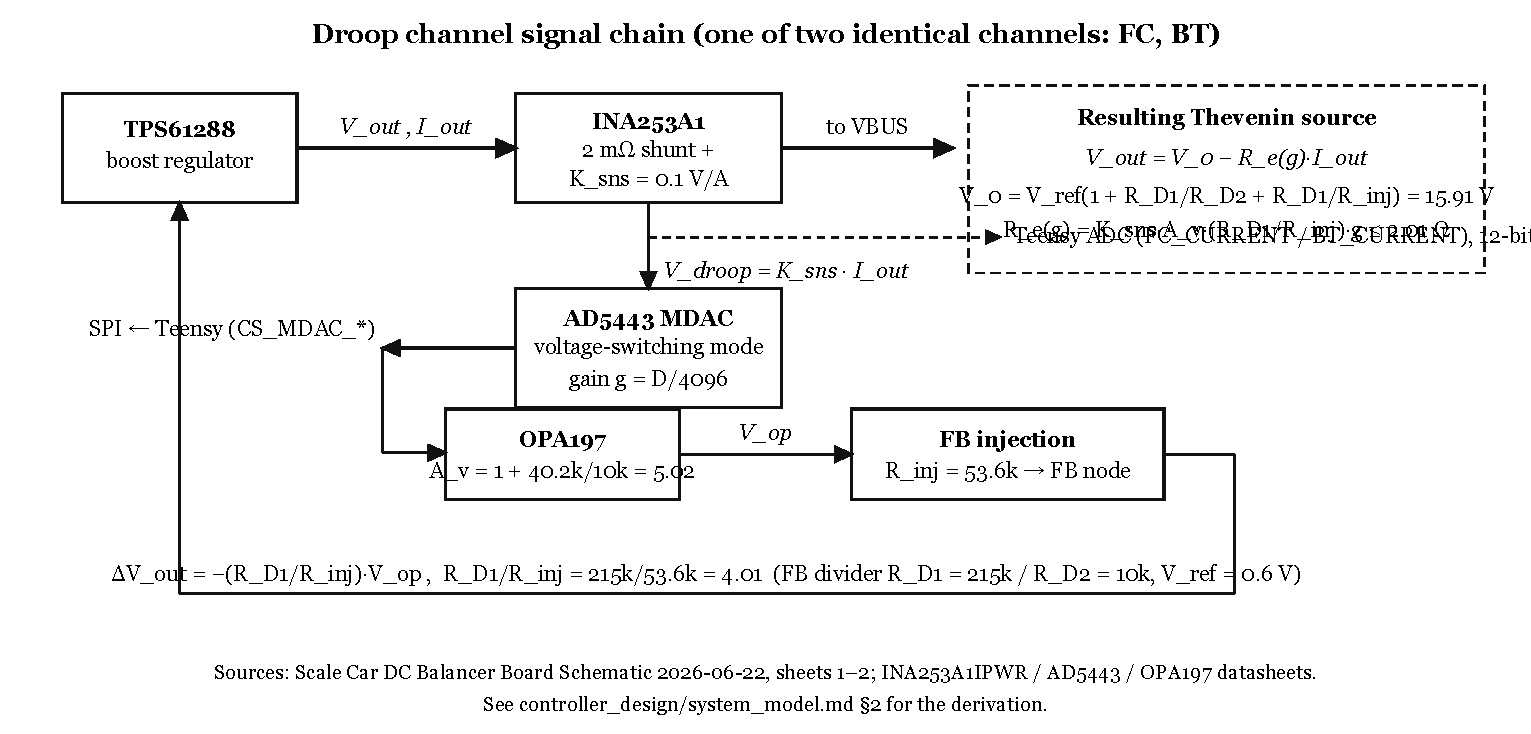
\includegraphics[width=\linewidth]{Figures/droop_signal_chain.pdf}
  \caption{Per-channel droop signal chain. The channel output current is sensed by the
  INA253A1 ($K_{sns}=0.1$\,V/A), scaled by the AD5443 MDAC (gain $g \in [0,4095/4096]$,
  written over SPI), amplified by the OPA197 ($A_v = 5.02$), and injected through
  $R_{inj}=53.6$\,k$\Omega$ into the TPS61288 feedback node
  ($R_{D1}=215$\,k$\Omega$, $R_{D2}=10$\,k$\Omega$). The converter is unmodified; the
  entire droop mechanism is an additive perturbation of its feedback divider.}
  \label{fig:droop-chain}
\end{figure}

\subsection{Droop Equations and the Actuator Mapping}
\label{sec:droop:equations}

\subsubsection{Effective output resistance}

The converter servos its feedback node to $V_{ref}$. Writing KCL at that node (feedback
pin current negligible) with the injected voltage $V_{op}$ gives

\begin{equation}
  \frac{V_{out}-V_{ref}}{R_{D1}} + \frac{V_{op}-V_{ref}}{R_{inj}} = \frac{V_{ref}}{R_{D2}},
  \label{eq:fb-kcl}
\end{equation}

which rearranges into an explicit Th\'evenin form,

\begin{equation}
  V_{out} = \underbrace{V_{ref}\!\left(1 + \frac{R_{D1}}{R_{D2}} + \frac{R_{D1}}{R_{inj}}\right)}_{V_0\ \text{(no-load setpoint)}}
            \;-\; \frac{R_{D1}}{R_{inj}}\,V_{op}.
  \label{eq:thevenin}
\end{equation}

Substituting the measured-current path $V_{op} = A_v\,g\,K_{sns}\,I_{out}$ yields the
programmable output resistance that is the heart of the scheme:

\begin{equation}
  V_{out} = V_0 - R_e(g)\,I_{out},
  \qquad
  \boxed{\;R_e(g) = K_{sns}\,A_v\,\frac{R_{D1}}{R_{inj}}\,g \;=\; R_{e,max}\,g\;}
  \label{eq:re}
\end{equation}

with the numerical values of the as-built board:

\begin{align}
  K_{sns} &= 0.1\ \mathrm{V/A}  && \text{INA253A1 fitted (A3 would be 0.4)}\\ % INA253A1IPWR.pdf; system_model.md §8
  A_v     &= 1 + \tfrac{40.2\,\mathrm{k}}{10\,\mathrm{k}} = 5.02 && \text{op-amp gain}\\ % schematic ROP1/ROP2; system_model.md §8; .ino const float A_v
  R_{D1}/R_{inj} &= \tfrac{215\,\mathrm{k}}{53.6\,\mathrm{k}} = 4.011 && \text{injection attenuation}\\ % system_model.md §2/§8; .ino RD1_OVER_RINJ
  R_{e,max} &= 0.1 \times 5.02 \times 4.011 = \mathbf{2.014\ \Omega} && \\ % system_model.md §8; .ino RE_MAX
  V_0 &= 0.6 \times 26.51 = 15.91\ \mathrm{V} && \text{no-load setpoint} % V_ref=0.6V, TPS61288LRQQR.pdf §7.5; system_model.md §2
\end{align}

% NOTE(author): the RD1 value is a post-manufacturing bodge (237k -> 215k, both channels,
% 2026-07-11, part of the 16 V bus retune). The released schematic still prints 237k.
% Decide whether the paper documents the bodge explicitly or simply reports as-built
% values; recommend a single footnote rather than a digression.
The 12-bit MDAC resolves this into $\Delta R_e = R_{e,max}/4096 = 0.49$\,m$\Omega$ per LSB,
which is far below any effect the current sensing can resolve; MDAC quantisation is
therefore omitted from the linear model.

\subsubsection{Two sources in parallel}

With both channels conducting onto the bus through their ideal-diode switches, and total
load current $I_{tot}$,

\begin{equation}
  V_{bus} = V_{0F} - R_F I_F = V_{0B} - R_B I_B, \qquad I_F + I_B = I_{tot}.
\end{equation}

The design choice that makes this a well-conditioned control problem is to command the two
droop resistances \emph{reciprocally} from a single scalar ratio $r$, using a fixed design
droop scale $k_d$ (denoted \texttt{K\_DROOP} in firmware):

\begin{equation}
  R_F = \frac{k_d}{r}, \qquad R_B = \frac{k_d}{1-r}.
  \label{eq:ratio-map}
\end{equation}

This has the property $R_F \parallel R_B = k_d$ \emph{independently of} $r$: the bus's
aggregate droop stiffness is constant while the split is swept. The resulting share is

\begin{equation}
  \boxed{\;\alpha \;=\; \frac{I_F}{I_{tot}} \;=\; r \;+\; \underbrace{\frac{\Delta V_0\, r(1-r)}{k_d\, I_{tot}}}_{d\ \text{(output disturbance)}}\;}
  \label{eq:share}
\end{equation}

where $\Delta V_0 \equiv V_{0F}-V_{0B}$ is the channel-to-channel no-load setpoint
mismatch. Three consequences drive the controller design: the nominal static gain is
exactly unity ($\alpha = r$); setpoint mismatch enters as an additive output disturbance
that is worst at $r=0.5$ and at light load and scales as $1/k_d$; and the same mismatch
perturbs the plant gain,
$\partial\alpha/\partial r = 1 + \Delta V_0(1-2r)/(k_d I_{tot})$, which is carried into
synthesis as parametric gain uncertainty.

\subsubsection{The actuator mapping --- and a design lesson}
\label{sec:droop:bug}

Combining \eqref{eq:re} and \eqref{eq:ratio-map} gives the mapping the firmware must
implement:

\begin{equation}
  \boxed{\;g_F = \frac{k_d}{R_{e,max}\,r}, \qquad g_B = \frac{k_d}{R_{e,max}\,(1-r)}\;}
  \label{eq:g-map}
\end{equation}

% NOTE(author): this subsection is deliberately a confession. Reviewers of control papers
% reward honestly reported model-vs-hardware defects far more than a clean narrative, and
% it directly motivates why the plant was re-derived from the schematic rather than from
% the existing code. Keep it, but tighten the tone -- it currently reads as a lab notebook.
It is worth reporting that the original firmware did \emph{not} implement
\eqref{eq:g-map}. It used an equivalent-resistance constant $k_{eq}=0.45$\,$\Omega$ and
computed $g = k_{eq}/(r\,K_{sns}A_v)$ --- an expression that models the sense-and-amplify
path but silently \emph{omits the feedback-injection attenuation} $R_{D1}/R_{inj}$, at that
time $237\,\mathrm{k}/53.6\,\mathrm{k}=4.42$. The consequence is not a mild gain error. The
commanded gain becomes $g_F = 0.45/(0.502\,r) = 0.896/r$, which exceeds unity for every
$r < 0.896$; the SPI write routine clamps to full scale; and therefore across essentially
the whole commanded range \emph{both} MDACs sat pinned at $g=1$, giving
$R_F = R_B = R_{e,max}$ and a fixed $50/50$ share.

The control-theoretic reading is the important one: the loop was not badly tuned, it was
operating on a \textbf{zero-gain plant}. Any $\partial\alpha/\partial r$ was identically
zero over the operating range, so no choice of controller gains --- and the legacy design
used $K_p = K_i = 1$, which \eqref{eq:share} makes superficially plausible since the
nominal plant gain is unity --- could have produced closed-loop share authority. The defect
is invisible to a firmware unit test (the code computes what it says it computes), invisible
to a step response at fixed load (the share is stable, merely uncontrolled), and only
becomes obvious when the actuator mapping is re-derived from the schematic and the
saturation limit $g \le 1$ is checked explicitly. The lesson we draw, and recommend, is
that \emph{an actuator-range audit against the physical hardware constants should be a
mandatory step before any plant identification}: a saturated actuator and a well-behaved
plant are indistinguishable in closed-loop data.

\subsection{Gain Selection and the PCB Constraints It Imposed}
\label{sec:droop:gains}

% NOTE(author): this is the section that answers the "co-design" claim in the abstract.
% Make explicit that the resistor values were chosen *because* of the droop gain decision,
% not the other way round.
The droop gain choice is not a purely digital decision. Because $R_e$ is realised in
analog hardware, selecting $k_d$ simultaneously fixes MDAC range utilisation, op-amp
headroom, and the achievable share authority --- and those in turn dictated component
values on the PCB. The binding constraints are the following.

\paragraph{Constraint 1: MDAC saturation sets the ratio span.}
Since $g \le 1$, \eqref{eq:g-map} bounds the usable ratio range by
$k_d \le R_{e,max}\cdot\min(r_{min},\,1-r_{max})$. This is a direct trade of \emph{droop
stiffness against control authority}:

\begin{table}[H]
  \centering
  \caption{Droop-scale bound versus commanded ratio span, at $R_{e,max}=2.014\ \Omega$.
           The middle row is the shipped design point.}
           % Source: system_model.md §4 trade table (values rescaled to the 215k RD1 bodge)
  \label{tab:kd-tradeoff}
  \begin{tabular}{lcl}
    \toprule
    Ratio span $[r_{min},r_{max}]$ & max $k_d$ ($\Omega$) & Character \\
    \midrule
    $[0.10,\,0.90]$ & 0.201 & Wide authority, weak droop \\
    $\mathbf{[0.15,\,0.85]}$ & \textbf{0.302} & \textbf{Shipped: $k_d=0.30\ \Omega$, max $g=0.993$} \\
    $[0.20,\,0.80]$ & 0.403 & Strong droop, narrow authority \\
    \bottomrule
  \end{tabular}
\end{table}

% NOTE(author): 0.30 is still TODO(calibrate) in firmware pending the CAL-1/CAL-3 bench runs.
% Either report it as provisional or hold the paper's number until bench data lands.
The selected point is $k_d = 0.30\ \Omega$ with clamps
$[\texttt{DROOP\_R\_MIN},\texttt{DROOP\_R\_MAX}] = [0.15,\,0.85]$, leaving $0.7\%$ of MDAC
range as margin against component tolerance. Larger $k_d$ suppresses the mismatch
disturbance $d \propto 1/k_d$ but costs bus regulation --- the droop sag at $r=0.5$ is
$k_d I_{tot}$, i.e.\ $1.8$\,V at $6$\,A --- and narrows the reachable share range. Smaller
$k_d$ widens authority but lets the $\Delta V_0$ mismatch dominate the share error.

\paragraph{Constraint 2: the injection resistor sets $R_{e,max}$ \emph{and} the bus setpoint
simultaneously.}
$R_{inj}$ appears in both \eqref{eq:thevenin} and \eqref{eq:re}: it attenuates the
injected droop signal (setting the ceiling $R_{e,max}$) and it also loads the feedback
divider (shifting the no-load setpoint $V_0$). It cannot be chosen for droop range alone.
The board's $R_{inj} = 53.6$\,k$\Omega$ against $R_{D1} = 215$\,k$\Omega$ yields
$R_{e,max}=2.014\ \Omega$ --- comfortably above the $0.302\ \Omega$ requirement, i.e.\ the
design deliberately uses only $\approx 15\%$ of the available droop authority at the range
centre so that the whole span stays clear of MDAC saturation. This coupling was also the
mechanism by which a later system-level decision propagated back into the droop design: the
$16$\,V bus retune (undertaken for converter overshoot headroom, unrelated to sharing)
changed $R_{D1}$ from $237$\,k to $215$\,k$\Omega$, which moved $R_{e,max}$ from
$2.220\ \Omega$ to $2.014\ \Omega$ and required $k_d$ to be reduced from $0.33$ to
$0.30\ \Omega$ to preserve the $g\le1$ bound.
% Source: .ino changelog lines 75-82; system_model.md §2 and §8.

\paragraph{Constraint 3: sense gain versus op-amp headroom.}
The OPA197 is supplied from the board's $5$\,V rail (a post-manufacturing change from
$3.3$\,V), so its output ceiling is $\approx 4.9$\,V. The injected signal is
$V_{op} = A_v g K_{sns} I_{out}$, so the headroom limit is
$g\,I_{out} \le 4.9/(5.02\times0.1) = 9.8$\,A --- non-binding for this vehicle, whose
per-channel current stays below roughly $3$\,A. Note, however, that this margin is a
\emph{consequence of a component substitution error}: the design intended the INA253A3
($K_{sns} = 0.4$\,V/A) and the INA253A1 ($0.1$\,V/A) was fitted. The A3 part would have
raised $R_{e,max}$ fourfold (making the MDAC range constraint far looser) but would equally
have reduced the headroom ceiling to $2.4$\,A$\cdot$g, which \emph{would} have been binding
at peak current. The firmware carries $K_{sns}$ as an explicit named constant precisely so
this variant choice remains a single-line change if the board is respun.
% Source: CLAUDE.md §5 and §7; system_model.md §8; .ino const float K_sns

\paragraph{Constraint 4: the clamps are the anti-windup boundary.}
Because the ratio clamps $[0.15,0.85]$ are the true actuator saturation, they --- not an
arbitrary controller output limit --- define the anti-windup boundary for the outer
share controller. The clamp is applied in the firmware before the mapping
\eqref{eq:g-map} is evaluated, so the commanded MDAC gain is guaranteed to satisfy
$g \le 1$ by construction and the digital controller never operates against a hidden
hardware limit. The legacy $[0.01,\,0.99]$ clamps, which permitted the saturated regime of
Section~\ref{sec:droop:bug}, were removed from the droop path.

Figure~\ref{fig:control-loop} places these elements in the linearised design loop used for
synthesis, showing where the mismatch disturbance $d$ and the current-sense noise $n$ enter.

\begin{figure}[H]
  \centering
  % FIGURE FILE: controller_design/figures/control_loop_model.svg
  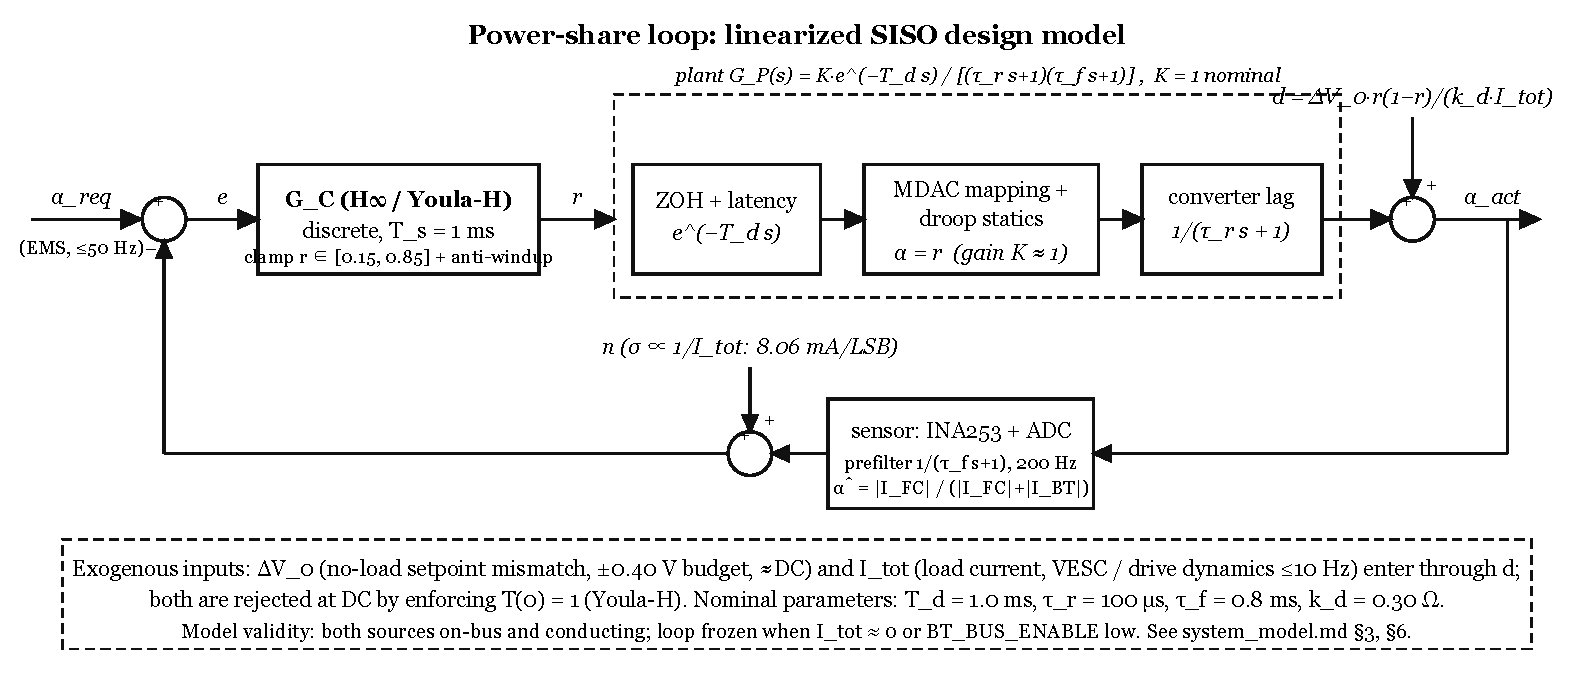
\includegraphics[width=\linewidth]{Figures/control_loop_model.pdf}
  \caption{Linearised SISO share-control loop. The controller commands the droop ratio $r$;
  the actuator mapping $g=k_d/(R_{e,max}r)$ and its clamp to $[0.15,0.85]$ form the
  saturation element. The plant reduces to a near-unity static gain in series with the
  converter lag $\tau_r$, the measurement prefilter $\tau_f$, and the dominant loop delay
  $T_d$. Setpoint mismatch $\Delta V_0$ enters as the additive output disturbance
  $d = \Delta V_0 r(1-r)/(k_d I_{tot})$; current-sense quantisation enters as output noise
  $n$ with variance scaling as $1/I_{tot}$.}
  \label{fig:control-loop}
\end{figure}

% =====================================================================
% PLANNING NOTES  (delete before submission)
% =====================================================================
% SCOPE / STATUS
% - This is a planning draft. Every number is traceable to
%   controller_design/system_model.md §2/§4/§8 or to the constants block in
%   teensy_controller/teensy_controller.ino (~lines 451-468). Do not edit numbers here
%   without editing system_model.md; that file is the declared source of truth.
%
% NUMBERS THAT ARE STILL PROVISIONAL (marked TODO(calibrate) in the repo)
% - k_d = 0.30 ohm  ..... bench decision pending (CAL-1 / CAL-3 in system_model.md §9).
%                         If it moves, Table \ref{tab:kd-tradeoff}, the 1.8 V sag figure,
%                         and the "0.7% MDAC margin" claim all change, AND the Youla-H
%                         controller coefficients must be regenerated (never hand-edited).
% - Delta V0 = +/-0.40 V  budgeted by tolerance RSS, not yet measured per board. The
%                         disturbance magnitudes quoted downstream depend on it.
% - tau_r = 100 us ...... lumped estimate; step test pending.
% - V_ref = 0.6 V ....... datasheet-verified (TPS61288 DS §7.5) but per-board value
%                         still to be measured in CAL-1.
%
% VERSION HAZARD -- READ BEFORE REUSING TEXT
% - Two sets of droop constants exist in the project history:
%     pre-retune  (RD1 = 237k): RE_MAX = 2.220 ohm, K_DROOP = 0.33, bound 0.3329
%     as-built    (RD1 = 215k): RE_MAX = 2.014 ohm, K_DROOP = 0.30, bound 0.3020
%   This section uses the AS-BUILT set throughout and mentions 2.220/0.33 only in
%   Constraint 2 as the superseded value. Earlier drafts and slide decks may quote the
%   pre-retune numbers. Cross-check any imported figure.
% - The released schematic (2026-06-22) still prints RD1 = 237k and RC-BT = 27.4k. Both
%   were bodged post-manufacturing. If a schematic excerpt is reproduced as a figure it
%   must carry a correction note or the numbers will contradict this section.
%
% FIGURES
% - Both figures exist as SVG in controller_design/figures/. LaTeX needs PDF:
%     inkscape --export-type=pdf droop_signal_chain.svg control_loop_model.svg
%   then copy into Figures/. Confirm the SVGs were regenerated after the 215k bodge --
%   if they annotate 237k they are stale.
% - Consider a third figure: measured alpha vs commanded r, overlaying the saturated
%   legacy mapping (flat at ~0.5) against the corrected mapping (slope ~1). That single
%   plot carries the Section \ref{sec:droop:bug} argument better than the prose does. Data
%   comes from the CAL-1 open-loop sweep (State 98 'O' command) -- NOT YET COLLECTED.
%
% PROSE TO REWRITE (see inline % NOTE markers)
% - Opening of \ref{sec:droop:ethos}: too terse, needs the paper's framing of the contribution.
% - \ref{sec:droop:bug}: currently reads as a lab notebook. Keep the honesty, raise the register.
% - \ref{sec:droop:gains} preamble: must land the hardware/control co-design claim explicitly.
%
% CROSS-REFERENCES TO WIRE UP
% - Constraint 4 -> the anti-windup discussion in the controller synthesis section.
% - Eq \eqref{eq:share} gain-uncertainty term -> the plant uncertainty set K in [0.75,1.25]
%   (widening to [0.55,1.45] at the ratio-span edges) used for synthesis.
% - The MDAC quantisation dismissal -> the noise budget section (system_model.md §5b).
%
% DELIBERATELY OUT OF SCOPE HERE
% - Converter-loop dynamics / tau_r justification (system_model.md §6e) and the
%   full-order validation (full_order_validation.md) belong in the plant-model section.
% - The RC-BT 27.4k -> 61.2k compensator bodge is a converter-symmetry issue, not a droop
%   gain issue; mention it only where the shared tau_r assumption is defended.
% =====================================================================
        % Droop ethos, gain calculations, PCB design constraints
% ============================================================================
% Section: Robust Power-Share Controller Design
% Uses amsmath, graphicx, booktabs, siunitx (loaded in main file).
% All numeric values carry a % comment citing the source file under
% controller_design/. Prose marked % NOTE is placeholder for the human author.
% ============================================================================

\section{Robust Power-Share Controller Design}
\label{sec:robust}

% NOTE (author): opening paragraph is a placeholder skeleton -- rewrite to connect
% back to the EMS section and to state the thesis contribution in one sentence.
The energy-management supervisor running on the vehicle's companion computer emits a
requested power-share $\alpha_{req}\in[0,1]$ at up to \SI{50}{\hertz}. Realising that
request on hardware is the job of an inner loop that adjusts the analogue droop
resistance of each of the two boost converters until the measured current split matches
the request. This section derives the plant seen by that loop, argues why a
nominal-tuned PI controller is inadequate for it, synthesises a robust replacement by
$\mathcal{H}_\infty$ mixed-sensitivity design followed by a Youla parameterisation gain
adjustment, and validates the result against both a 60-corner uncertainty family and an
independently constructed full-order converter model.

% ---------------------------------------------------------------------------
\subsection{Plant Model of the Droop-Controlled Share Loop}
\label{sec:share-plant}

% NOTE(orchestrator): the droop chain derivation and Eq. (share law) also appear in
% Section \ref{sec:droop}. In the final paper keep the full derivation in Sec. 2 and
% reduce this subsection to the *dynamic* modeling (design plant, corners), citing
% back. Kept in full here so each section reads standalone during planning.

\subsubsection{Per-channel programmable output resistance}

Each source channel (fuel cell, FC; battery, BT) is a synchronous boost converter whose
output voltage is drooped in analogue hardware in proportion to its own output current.
The sensed current passes through a current-sense amplifier of gain
$K_{sns}=\SI{0.1}{\volt\per\ampere}$, % system_model.md §8 (INA253A1IPWR fitted, A1 variant)
a 12-bit multiplying DAC of programmable gain $g\in[0,1]$, and a non-inverting stage of
gain $A_v = 1 + R_{op2}/R_{op1} = \num{5.02}$, % system_model.md §2 (R_op1=10k, R_op2=40.2k)
and is then injected into the regulator feedback node through $R_{inj}=\SI{53.6}{\kilo\ohm}$
against the divider $R_{D1}=\SI{215}{\kilo\ohm}$, $R_{D2}=\SI{10}{\kilo\ohm}$.
% system_model.md §8: R_D1 bodged 237k -> 215k on both channels (16 V bus retune, 2026-07-11)
Applying Kirchhoff's current law at the feedback node, which the regulator servos to
$V_{ref}$, gives a Th\'evenin source with an \emph{electronically programmable} output
resistance

\begin{equation}
V_{out} = V_0 - R_e(g)\,I_{out},
\qquad
R_e(g) = K_{sns}A_v\frac{R_{D1}}{R_{inj}}\,g \;=\; R_{e,max}\,g .
\label{eq:Re-robust}
\end{equation}

With the fitted values, $R_{D1}/R_{inj}=\num{4.0112}$, $V_0 = \SI{15.91}{\volt}$ and
$R_{e,max} = \SI{2.014}{\ohm}$, % system_model.md §2 and §8 (derived: K_sns·A_v·R_D1/R_inj)
giving a droop resolution of \SI{0.492}{\milli\ohm} per DAC code.
% system_model.md §2: ΔR_e = R_e,max/4096

% NOTE (author): the sentence below records a firmware defect found by this modelling
% exercise. It is told at length in Section \ref{sec:droop:bug}; here it is only a
% cross-reference. Decide which section owns the story.
The factor $R_{D1}/R_{inj}$ --- the attenuation of the injection path by the feedback
divider --- was omitted in the original firmware droop mapping, which therefore commanded
DAC gains $g>1$ over almost the entire ratio range and left both DACs clamped at full
scale. The share loop consequently saw a \emph{zero-gain} plant, a defect invisible to
any nominal-model simulation and only exposed by writing~\eqref{eq:Re-robust} out against
the schematic (Section~\ref{sec:droop:bug}).

\subsubsection{Two channels in parallel: the static share law}

Both Th\'evenin sources feed the DC bus through ideal-diode switches. With
$V_{bus}=V_{0F}-R_FI_F=V_{0B}-R_BI_B$ and $I_F+I_B=I_{tot}$, and adopting the
droop-ratio mapping $R_F = k_d/r$, $R_B = k_d/(1-r)$ --- for which the parallel droop
$R_F\!\parallel\!R_B = k_d$ is independent of $r$ --- the measured share obeys

\begin{equation}
\alpha \;\equiv\; \frac{I_F}{I_{tot}}
\;=\; r \;+\; \underbrace{\frac{\Delta V_0\,r(1-r)}{k_d\,I_{tot}}}_{d},
\qquad \Delta V_0 \equiv V_{0F}-V_{0B}.
\label{eq:share-static}
\end{equation}

Three structural facts follow, and they set the entire control problem.

\begin{enumerate}
\item \textbf{The nominal static gain is exactly unity} ($\alpha=r$ when $\Delta V_0=0$),
by construction of the $k_d/r$ mapping. This is precisely why a PI controller with
$K_p=K_i=1$ appeared adequate on paper.
\item \textbf{Set-point mismatch enters as an additive output disturbance} $d$, worst at
$r=0.5$ and at light load, and inversely proportional to the droop scale $k_d$. With a
plausible per-board $\Delta V_0 = \SI{0.4}{\volt}$ and $k_d = \SI{0.30}{\ohm}$,
$d = 0.33/I_{tot}$, i.e.\ \textbf{0.17 share at \SI{2}{\ampere}}. % system_model.md §5a
This is a very large static offset and is the reason exact integral action is a hard
requirement rather than a refinement.
\item \textbf{The same mismatch perturbs the plant gain},
$\partial\alpha/\partial r = 1 + \Delta V_0(1-2r)/(k_d I_{tot})$, which is treated as
parametric gain uncertainty $K\in[1-\delta,1+\delta]$.
\end{enumerate}

The actuator constraint $g\le 1$ bounds the usable authority:
$k_d \le R_{e,max}\min(r_{min},1-r_{max})$. The design adopts
$r\in[\num{0.15},\num{0.85}]$ with $k_d=\SI{0.30}{\ohm}$ (hard bound \SI{0.3020}{\ohm}),
% system_model.md §4 trade table
which trades a \SI{1.8}{\volt} bus sag at \SI{6}{\ampere} against a manageable mismatch
disturbance. Twelve-bit DAC quantisation moves the share by $\approx\num{3.7e-5}$ per
code at the range edge and is negligible against the sensor noise floor.
% system_model.md §4 quantization paragraph

\subsubsection{Dynamics and the design plant}

The share statics are, remarkably, \emph{instantaneous}: with $\Delta V_0=0$ both channel
currents carry the common factor $(V_0-V_{bus}(t))$, so
$\alpha(t) = G_F/(G_F+G_B) = r$ at every instant regardless of the bus-voltage transient.
% system_model.md §6a
The bus-capacitance pole therefore appears in the share response only through the
mismatch term, with residue $\propto \Delta V_0/(k_dI_{tot})$, and is absorbed into the
uncertainty description rather than modelled explicitly. What remains is the digital
layer plus the converter voltage loops, giving the design plant

\begin{equation}
G_P(s) \;=\; \frac{K\,e^{-T_d s}}{(\tau_r s + 1)(\tau_f s + 1)} .
\label{eq:design-plant}
\end{equation}

\begin{table}[H]
\caption{Design-plant parameters and uncertainty ranges.}
\label{tab:plant-params}
\begin{tabular}{llll}
\toprule
\textbf{Parameter} & \textbf{Nominal} & \textbf{Range} & \textbf{Physical origin}\\
\midrule
$K$      & 1                  & $[0.55,\ 1.45]$          & static mismatch gain term, Eq.~\eqref{eq:share-static}\\
$T_d$    & \SI{1.0}{\milli\second} & $[0.5,\ 2.0]$~ms    & zero-order hold $+$ compute-to-apply latency at $T_s=\SI{1}{\milli\second}$\\
$\tau_r$ & \SI{100}{\micro\second} & $[20,\ 300]$~\textmu s & converter voltage-loop lag, lumped with sense and bus parasitics\\
$\tau_f$ & \SI{0.8}{\milli\second} & $\{0,\ 0.8\}$~ms    & optional \SI{200}{\hertz} measurement prefilter\\
\bottomrule
\end{tabular}
\end{table}
% Table values: system_model.md §6d. Wide K set [0.55,1.45] applies at the r-range edges
% with the full ±0.4 V mismatch budget; [0.75,1.25] holds for r∈[0.3,0.7] at I_tot ≥ 2 A.

The loop delay budget is $T_d = T_s/2 + T_s + \varepsilon \approx \SI{1.5}{\milli\second}$
worst case at the chosen \SI{1}{\kilo\hertz} rate, which gives $\ge 20\times$
oversampling of the intended \SIrange{5}{10}{\hertz} closed-loop bandwidth while leaving
the fast firmware tick free for fault detection and motor control.
% system_model.md §6c

The plant is thus \emph{delay-dominated with near-unity gain}. The lumping of the two
converter voltage loops into the single lag $\tau_r$ is justified by time-scale
separation of about \num{2.5} decades: the converter loops cross at
\SIrange{6}{22}{\kilo\hertz} (from datasheet compensator arithmetic with
$R_C=\SI{61.2}{\kilo\ohm}$ on \emph{both} channels), % system_model.md §6e
whereas the share loop crosses near \SI{110}{\radian\per\second}. Even the slowest
modelled $\tau_r=\SI{300}{\micro\second}$ contributes only $\ang{1.9}$ of phase at the
share crossover. Section~\ref{sec:fullorder} replaces this argument with empirical
evidence.

% ---------------------------------------------------------------------------
\subsection{Why Robustness, and Not Tuning, Is the Issue}
\label{sec:why-robust}

% NOTE (author): this subsection carries the paper's argument. Rewrite the prose freely,
% but keep the 26.9 vs 1.87 comparison as the headline claim -- it is the single number
% that justifies the whole design effort.
Equation~\eqref{eq:share-static} makes the plant look trivial: unity DC gain, one small
lag, one small delay. That appearance is exactly the trap. The unity gain is a property
of the \emph{nominal} hardware, and the two channels are not nominally identical in
practice:

\begin{itemize}
\item \textbf{Regulator tolerance bands are wide.} The converter feedback reference is
specified over \SIrange{0.588}{0.612}{\volt} across process and temperature ($\pm\SI{2}{\percent}$),
% system_model.md §5a, TPS61288LRQQR.pdf §7.5
and with $\pm\SI{1}{\percent}$ divider resistors the channel-to-channel no-load voltage
difference budgets to $\pm\SI{3.4}{\percent}$, i.e.\ $\Delta V_0 \approx \pm\SI{0.6}{\volt}$
worst case. Through Eq.~\eqref{eq:share-static} this is simultaneously a large output
disturbance \emph{and} a plant-gain perturbation.
\item \textbf{Ceramic output capacitance derates strongly with bias.} The three
\SI{22}{\micro\farad} output capacitors present \SI{66}{\micro\farad} nominally but
$\approx\SI{30}{\micro\farad}$ derated, % full_order_validation.md §3 envelope axes
which moves each converter's voltage-loop crossover by better than a factor of two and
hence moves $\tau_r$.
\item \textbf{The right-half-plane zero moves with load and duty.} $f_{RHPZ}$ ranges over
\SIrange{31}{330}{\kilo\hertz} across the \SIrange{2}{8}{\ampere} load envelope,
% system_model.md §6e item 2
so the converter dynamics that the lump is meant to cover are themselves operating-point
dependent.
\item \textbf{The channels are asymmetric by construction.} They run from different input
voltages (\SIrange{9}{12}{\volt} fuel-cell side versus \SIrange{7.4}{8.4}{\volt} battery
side), % system_model.md §6e table
so their duty cycles, RHP zeros and crossovers differ even with identical components.
Matching the compensator resistor across the two channels was a deliberate hardware
change made \emph{so that} a single shared $\tau_r$ would be defensible.
\item \textbf{Measurement noise scales as $1/I_{tot}$.} One ADC code is
\SI{8.06}{\milli\ampere}, % system_model.md §5b (SCALE_I)
so the share measurement quantises at \SI{0.4}{\percent} at \SI{2}{\ampere} but
\SI{1.6}{\percent} at \SI{0.5}{\ampere}, requiring high-frequency roll-off of the actuator
signal to avoid DAC chatter.
\end{itemize}

A controller tuned at the nominal point cannot be assumed to survive this set, and in
this case it does not. Evaluated on the discrete closed loop over the parameter corners
of Table~\ref{tab:plant-params}, the legacy $K_p=K_i=1$ PI reaches a peak sensitivity of
$\|S\|_\infty = \num{26.9}$ (\SI{28.6}{\decibel}), whereas the robust design developed
below peaks at $\|S\|_\infty = \num{1.87}$ (\SI{5.4}{\decibel}).
% synthesis_metrics.txt: "discrete worst ||S||inf: youla = 1.867, legacy PI = 26.889"
A sensitivity peak of \num{26.9} corresponds to a disk margin so small that the loop is,
for engineering purposes, conditionally stable at the corners --- and the corners here
are not exotic: they are a cold board, a derated capacitor, and two converters from
different reels. This factor-of-\num{14} gap in worst-case sensitivity peak, not any
improvement in nominal step response, is the justification for a robust synthesis.

% ---------------------------------------------------------------------------
\subsection{\texorpdfstring{$\mathcal{H}_\infty$}{H-infinity} Synthesis and Youla-H Gain Adjustment}
\label{sec:synthesis}

\subsubsection{Mixed-sensitivity problem and weight selection}

The controller is synthesised by mixed-sensitivity $\mathcal{H}_\infty$ design on the
stacked $S/KS/T$ problem, followed by the Youla-H post-synthesis gain adjustment of
Tan et~al.\ that enforces exact unity DC complementary sensitivity.
% controller_synthesis.md header: method = Tan, Yadav, Assadian 2026
The delay is represented by a second-order Pad\'e approximant, so the nominal augmented
plant has four states.

\begin{table}[H]
\caption{Synthesis weights and their design intent.}
\label{tab:weights}
\begin{tabular}{llll}
\toprule
\textbf{Weight} & \textbf{Acts on} & \textbf{Form / values} & \textbf{Intent}\\
\midrule
$W_p$ & $S$ & strictly proper $Ma/(s+a)$, $M=10^4$, unity crossing \SI{40}{\radian\per\second} & integral-action pressure; disturbance rejection below \SI{40}{\radian\per\second}\\
$W_d$ & $T$ & \texttt{makeweight(0.5, 250, 40)} & force $T$ roll-off above \SI{250}{\radian\per\second} (noise, unmodelled HF)\\
$W_u$ & $Y$ & \texttt{makeweight(0.3, 600, 20)} & cap actuator effort; roll off DAC activity above \SI{600}{\radian\per\second}\\
\bottomrule
\end{tabular}
\end{table}
% Weight table: controller_synthesis.md §2

$W_p$ is deliberately chosen \emph{strictly} proper. Since $S\to 1$ at high frequency
needs no penalty, this costs nothing in design terms but makes the augmented plant
satisfy $D_{11}=0$ exactly, so the regular DGKF problem applies and the estimation
Riccati equation degenerates analytically ($D_{21}=1 \Rightarrow Q_y=0$, $A-B_1C_2$
stable $\Rightarrow Y=0$), leaving a single Riccati solve and the central controller
$\dot{\hat{x}} = (A-B_1C_2+B_2F)\hat{x} + B_1e$, $u=F\hat{x}$.
% controller_synthesis.md §1
% NOTE (author): the following sentence is a methods disclosure -- keep or cut depending
% on whether the venue wants reproducibility detail at this level.
Because no commercial robust-control toolbox was available on the development machine,
the Riccati solutions were computed from the Hamiltonian matrix by ordered real Schur
decomposition with $\gamma$-iteration by bisection, in a purpose-written implementation
whose primitives are unit-tested against reference solvers and whose every synthesised
controller passes an \emph{a-posteriori} gate: closed-loop stability plus
$\|T_{zw}\|_\infty \le \gamma$ evaluated by an independent Hamiltonian-bisection norm.
A derivation error therefore cannot silently yield an accepted controller.

\subsubsection{Synthesis result and the \texorpdfstring{$T(0)=1$}{T(0)=1} step}

\begin{table}[H]
\caption{Synthesis outcome (nominal plant).}
\label{tab:synth-results}
\begin{tabular}{ll}
\toprule
\textbf{Quantity} & \textbf{Value}\\
\midrule
$\gamma_{opt}$                                 & \num{0.6532}\\          % synthesis_metrics.txt
Controller built at                            & $\gamma=\num{0.6859}$ (\SI{5}{\percent} back-off), $\|T_{zw}\|_\infty=\num{0.6841}$ \checkmark\\ % synthesis_metrics.txt
$\mathcal{H}_\infty$ controller order          & 7 (4 plant $+$ 3 weight states)\\ % controller_synthesis.md §3
$T_H(0)$ before adjustment                     & \num{0.99996423}\\      % synthesis_metrics.txt
$T_{YH}(0)$ after adjustment                   & \num{1.000000000000}\\  % synthesis_metrics.txt
$S/T$ crossover                                & \SI{109.9}{\radian\per\second}\\ % synthesis_metrics.txt
$\|S\|_\infty,\ \|T\|_\infty,\ \|Y\|_\infty$   & \num{1.25}, \num{1.00}, \num{1.01}\\ % controller_synthesis.md §3
Nominal $M_2$ / phase margin / delay margin    & \num{0.7978} / \ang{73.9} / \SI{11.74}{\milli\second}\\ % synthesis_metrics.txt
\bottomrule
\end{tabular}
\end{table}

That $\gamma_{opt}<1$ with margin means every weighted specification is met, but the
$\mathcal{H}_\infty$ solution exhibits the classical DC deficiency: $T_H(0)=\num{0.99996423}$,
short of unity by \SI{0.0036}{\percent}. For this application that residual is not
cosmetic. It leaves a finite DC loop gain, so the static mismatch disturbance $d$ of
Eq.~\eqref{eq:share-static} --- which can be \num{0.17} in share at \SI{2}{\ampere} --- is
only attenuated, not rejected, and a ramping EMS reference accrues a persistent bias.

The Youla-H step applies the scalar gain correction $Y_{YH} = Y_H/T_H(0)$ and recovers
the controller as $G_{C,YH} = Y_{YH}(1-G_PY_{YH})^{-1}$.
% controller_synthesis.md §3
This \SI{+0.0036}{\percent} gain shift places an exact integrator in the controller: the
near-origin pole of $G_{C,YH}$ appears at $|p|=\num{5.6e-9}$ and is snapped to a true
integrator by the spectral split of the following subsection. The outcome is
$T(0)=1$ to machine precision, hence exact DC disturbance rejection and zero ramp-following
bias, obtained \emph{without} re-tuning the weights and without disturbing the
$\mathcal{H}_\infty$ robustness the synthesis just bought.

\begin{figure}[H]
\centering
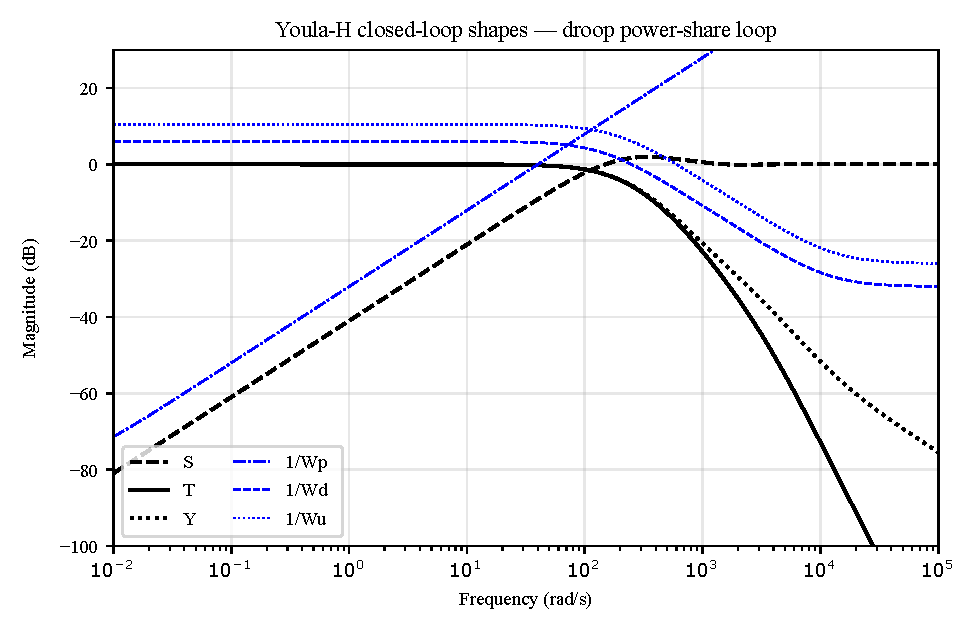
\includegraphics[width=\textwidth]{Figures/loopshapes_youla_h.pdf}
% source: controller_design/figures/loopshapes_youla_h.svg (data: loopshapes_youla_h.csv)
\caption{Achieved sensitivity $S$, complementary sensitivity $T$ and control sensitivity
$Y$ of the Youla-H design, plotted against the inverse weights $1/W_p$, $1/W_d$, $1/W_u$.
All three lie inside their templates, consistent with $\gamma_{opt}=\num{0.6532}$.}
\label{fig:loopshapes}
\end{figure}

\subsubsection{Order reduction, discretisation, and firmware realisation}

The controller is decomposed as $G_{C,YH}(s) = k_I/s + R(s)$ with
$k_I=\num{111.93}$ % synthesis_metrics.txt: kI = 111.929630
--- consistent with the observed crossover, since $|L|=1$ where $k_I/\omega\approx 1$ ---
and the 21-state stable remainder $R(s)$ is reduced by balanced truncation to
\textbf{three states}. The Hankel singular values (\num{14.8}, \num{0.035}, \num{0.0018},
\num{5e-5},~\ldots) % controller_synthesis.md §4
justify the cut, and the reduced controller's frequency response deviates from the full
one by at most \SI{0.8}{\percent}.

Tustin discretisation at $T_s=\SI{1}{\milli\second}$ yields three second-order sections
plus a trapezoidal integrator. The embedded implementation evaluates

\begin{equation}
u_k = r_0 + R(z)e_k + I(z)e_k, \qquad r_0 = 0.5,
\qquad r_k = \mathrm{sat}_{[r_{min},\,r_{max}]}(u_k),
\label{eq:ctrl-impl}
\end{equation}

as a cascade of Direct-Form-II-transposed biquads in single precision, with the output
clamped to $[\num{0.15},\num{0.85}]$. Anti-windup is by \textbf{back-calculation on the
output clamp}: when $u_k$ would leave the interval, the integrator state absorbs exactly
the excess, so the command sits on the rail and resumes moving on the tick the error
reverses. The biquad states are deliberately \emph{not} clamped --- $R(z)$ is stable and
cannot wind up, so clamping it would only introduce a spurious nonlinearity. The measured
share (only --- never the set-point) passes through the \SI{200}{\hertz} one-pole
prefilter that is part of the design plant as $\tau_f$, so EMS steps are not smoothed by
a sensor filter. A wrapper gates the update to exactly one execution per $T_s$ and holds
the output between ticks; that zero-order hold is itself accounted for in $T_d$.

Two implementation notes are worth recording. First, one discrete section carries a pole
at $z=\num{0.999996}$ --- the $W_p$ weight pole reappearing nearly cancelled in the
controller. Its distance from the unit circle, \num{4e-6}, is about $30\times$ single-
precision epsilon at unity, so the section is representable, and its Hankel singular value
(\num{0.035}) shows it genuinely contributes rather than being truncation noise.
% controller_synthesis.md §4 and §8
Second, the loop freezes (states held, no integration) when $I_{tot}\approx 0$, matching
the validity limit of Eq.~\eqref{eq:share-static}, where $\alpha$ is undefined.

\begin{figure}[H]
\centering
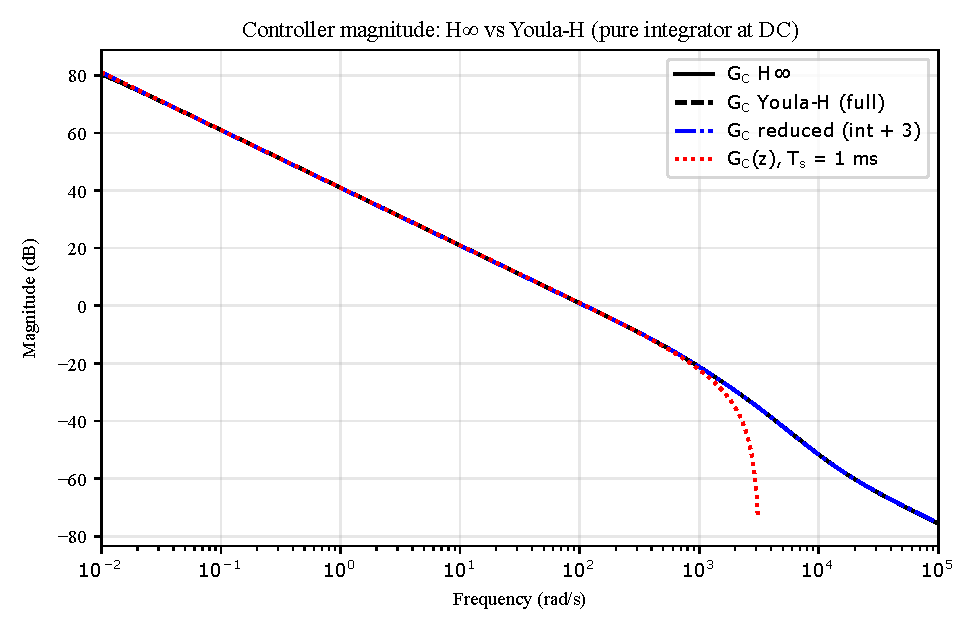
\includegraphics[width=\textwidth]{Figures/controller_bode.pdf}
% source: controller_design/figures/controller_bode.svg (data: controller_bode.csv)
\caption{Controller frequency response at each stage of the realisation: the raw
$\mathcal{H}_\infty$ controller, the Youla-H adjusted controller, the reduced
form, and the discretised implementation. The exact integrator introduced by
the Youla-H step is visible as the diverging low-frequency branch that the raw
$\mathcal{H}_\infty$ controller lacks.}
\label{fig:ctrl-bode}
\end{figure}

% ---------------------------------------------------------------------------
\subsection{Validation}
\label{sec:validation}

\subsubsection{Corner sweeps and time-domain behaviour}

The design was checked over the full uncertainty family of Table~\ref{tab:plant-params}:
$K\in\{0.55\ldots1.45\}$, $T_d\in\{0.5,1,2\}$~ms, $\tau_r\in\{20,300\}$~\textmu s,
$\tau_f\in\{0,0.8\}$~ms, i.e.\ \textbf{60 corners}. All 60 continuous-time closed loops
are stable, with worst-case $M_2=\num{0.5905}$ occurring at $(K,T_d,\tau_r,\tau_f) =
(\num{1.45}, \SI{2}{\milli\second}, \SI{300}{\micro\second}, \SI{0.8}{\milli\second})$;
% synthesis_metrics.txt: worst-corner M2 = 0.5905 at (1.45, 0.002, 0.0003, 0.0008)
the corresponding discrete sweep (zero-order-hold plant against the \emph{implemented}
$G_C(z)$) has all closed-loop poles inside the unit circle.

\begin{table}[H]
\caption{Validation summary. All entries generated by the synthesis pipeline.}
\label{tab:validation}
\begin{tabular}{lll}
\toprule
\textbf{Check} & \textbf{Result} & \textbf{Source}\\
\midrule
Continuous 60-corner sweep      & all stable, worst $M_2=\num{0.5905}$          & \texttt{synthesis\_metrics.txt}\\
Discrete 60-corner sweep        & all $|z|<1$                                    & \texttt{synthesis\_metrics.txt}\\
Nominal margins                 & GM \SI{18.5}{\decibel}, PM \ang{73.9} at \SI{110}{\radian\per\second}, delay margin \SI{11.74}{\milli\second} & \texttt{MATLAB\_validation.txt}\\
Step $0.5\to0.7$ (discrete)     & \SI{2}{\percent} settle \SI{22}{\milli\second}, \SI{0}{\percent} overshoot, SS error \num{8e-9} & \texttt{synthesis\_metrics.txt}\\
Ramp \SI{0.05}{\per\second}     & tracking error \num{4.47e-4}, no accumulating bias & \texttt{synthesis\_metrics.txt}\\
Anti-windup (\SI{0.5}{\second} into the rail) & leaves rail $\le 3$ ticks after error reversal, recovery $<\SI{150}{\milli\second}$ & \texttt{controller\_synthesis.md} §5\\
Worst-corner discrete $\|S\|_\infty$ & \textbf{\num{1.867}} (legacy PI: \num{26.889}) & \texttt{synthesis\_metrics.txt}\\
\bottomrule
\end{tabular}
\end{table}

The delay margin of \SI{11.74}{\milli\second} deserves emphasis: it is roughly
$6\times$ the worst \emph{modelled} loop delay of \SI{2}{\milli\second}. Since the timing
parameters are pre-calibration estimates, this margin --- not any single nominal number
--- is what makes the design safe to commit to firmware ahead of bench identification.

\begin{figure}[H]
\centering
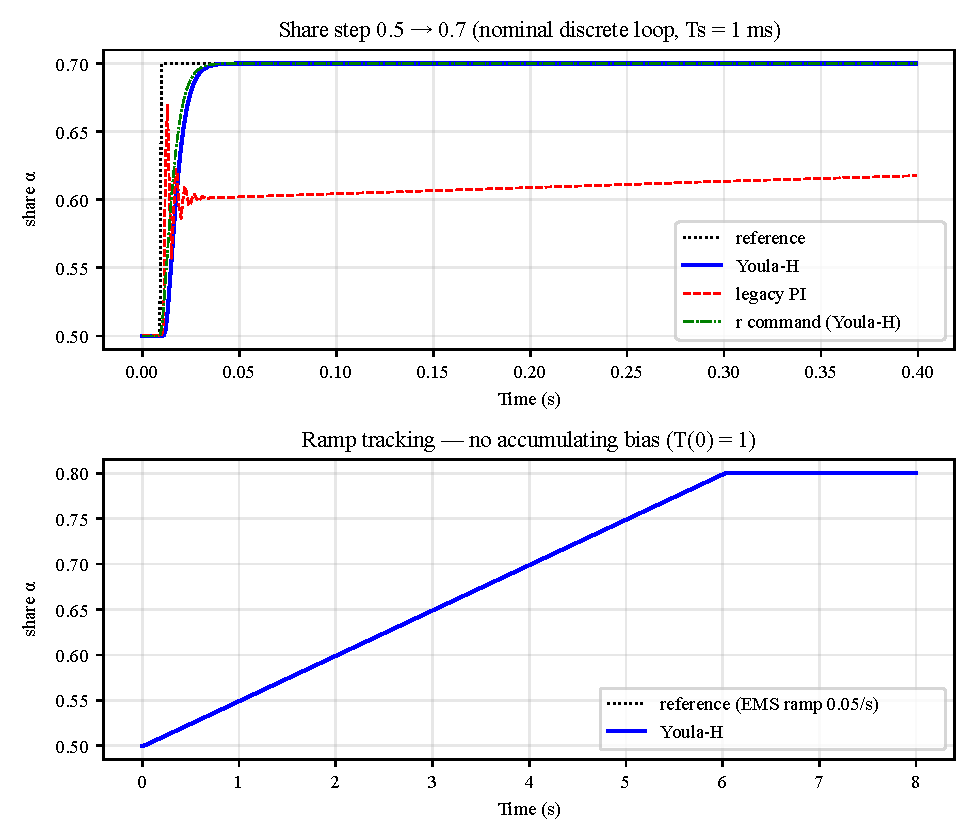
\includegraphics[width=\textwidth]{Figures/timedomain_step_ramp.pdf}
% source: controller_design/figures/timedomain_step_ramp.svg (data: timedomain_step_ramp.csv)
\caption{Discrete-time closed-loop response of the implemented controller: share step
$0.5\to0.7$ (left) and ramp reference at \SI{0.05}{\per\second} (right). The ramp
panel is the practical expression of $T(0)=1$: the tracking error decays to
\num{4.5e-4} instead of settling to a constant offset.}
\label{fig:timedomain}
\end{figure}

\begin{figure}[H]
\centering
% TODO(figure): no rendered figure exists yet — plot from
% controller_design/figures/step_response_nominal.csv and step_response_mismatch.csv
% (columns: t_s, r_cmd, alpha, v_bus).
\fbox{\parbox[c][4cm][c]{0.9\textwidth}{\centering PLACEHOLDER --- plot from
\texttt{step\_response\_nominal.csv} / \texttt{step\_response\_mismatch.csv}}}
\caption{Open-loop verification of the static share law, Eq.~\eqref{eq:share-static},
from the independent numerical model: commanded ratio $r$, achieved share $\alpha$, and
bus voltage. With matched channels ($\Delta V_0 = 0$) the share tracks $r$ instantaneously;
the companion mismatch case ($\alpha = \num{0.48}$ at $r = \num{0.40}$) shows the
open-loop offset that only integral action can remove.}
\label{fig:step-openloop}
\end{figure}

\subsubsection{Full-order cross-validation}
\label{sec:fullorder}

The design plant~\eqref{eq:design-plant} rests on lumping two converter voltage loops into
one uncertain lag. To test that reduction rather than merely argue it, a complete
small-signal model of the share plant was constructed \emph{independently}: both channels'
transconductance-amplifier compensators with the exact COMP-node impedance
$Z_{comp}=R_{EA}\|(R_C+1/sC_C)\|1/sC_P$, Norton-equivalent power stages carrying the
right-half-plane and ESR zeros, the three-resistor feedback node with the bilinear droop
injection linearised at $(g_0,I_0)$, current-sense dynamics, bus coupling, and the same
digital layer --- \textbf{11 states} per operating point, against two states plus a delay
in the design model.
% full_order_validation.md §1.1-1.4

Structural gate checks confirm the construction before any comparison is drawn: the
Norton form reduces to the datasheet power-stage expression to machine precision
($\num{4.5e-16}$); the DC share gain emerging from the full linearisation is \num{0.9933},
short of unity only by the finite error-amplifier DC gain; and the per-channel voltage-loop
crossovers reproduce the independent datasheet arithmetic to within \SIrange{1}{3}{\percent}
(e.g.\ FC \SI{16.33}{\kilo\hertz} computed versus \SI{16.84}{\kilo\hertz} predicted).
% full_order_validation.md §2, gates A/B/C

\begin{table}[H]
\caption{Full-order versus simplified plant, and closed-loop equivalence with the shipped
controller.}
\label{tab:fullorder}
\begin{tabular}{lll}
\toprule
\textbf{Check} & \textbf{Full-order model} & \textbf{Simplified model}\\
\midrule
Nominal in-band deviation ($\omega\le\SI{1100}{\radian\per\second}$) & \SI{3.86}{\percent} & --- \\
Envelope deviation, 432 operating points & \SI{5.78}{\percent} worst, \SI{4.30}{\percent} median & ---\\
Discrete closed-loop stability & \textbf{432/432} points & 60/60 corners\\
Worst discrete $\|S\|_\infty$ & \textbf{\num{1.240}} & \num{1.867}\\
Step $0.5\to0.7$ overlay & max divergence \num{0.0008} share & ---\\
\SI{2}{\percent} settle & \SI{25}{\milli\second} & \SI{22}{\milli\second}\\
Ramp error at \SI{3}{\second} & \num{4.30e-4} & \num{4.47e-4}\\
\bottomrule
\end{tabular}
\end{table}
% All entries: fullorder_metrics.txt

The 432-point envelope spans $\{V_{in,FC}\;9/12\}\times\{V_{in,BT}\;7.4/8.4\}\times
\{I_{tot}\;1/2/4\,\mathrm{A}\}\times\{r_0\;0.3/0.5/0.7\}\times\{C_O\;30/66\,\mu\mathrm{F}\}
\times\{C_{bus}\;30/500\,\mu\mathrm{F}\}\times\{R_{EA}\;1/10/100\,\mathrm{M}\Omega\}$;
% full_order_validation.md §3
the amplifier output resistance is swept rather than assumed because the datasheet does
not specify it, converting a hidden assumption into a verified non-sensitivity.

Two results matter. First, every full-order response lies within \SI{5.78}{\percent} of
\emph{some} member of the simplified corner family, so the uncertainty set used for
synthesis was a genuine superset of the true dynamics. Second, the worst full-order
closed-loop sensitivity peak (\num{1.240}) is \emph{lower} than the simplified family's
worst (\num{1.867}) --- the expected sign, confirming that the corner family was
pessimistic in the safe direction rather than accidentally optimistic in some unmodelled
one.

\begin{figure}[H]
\centering
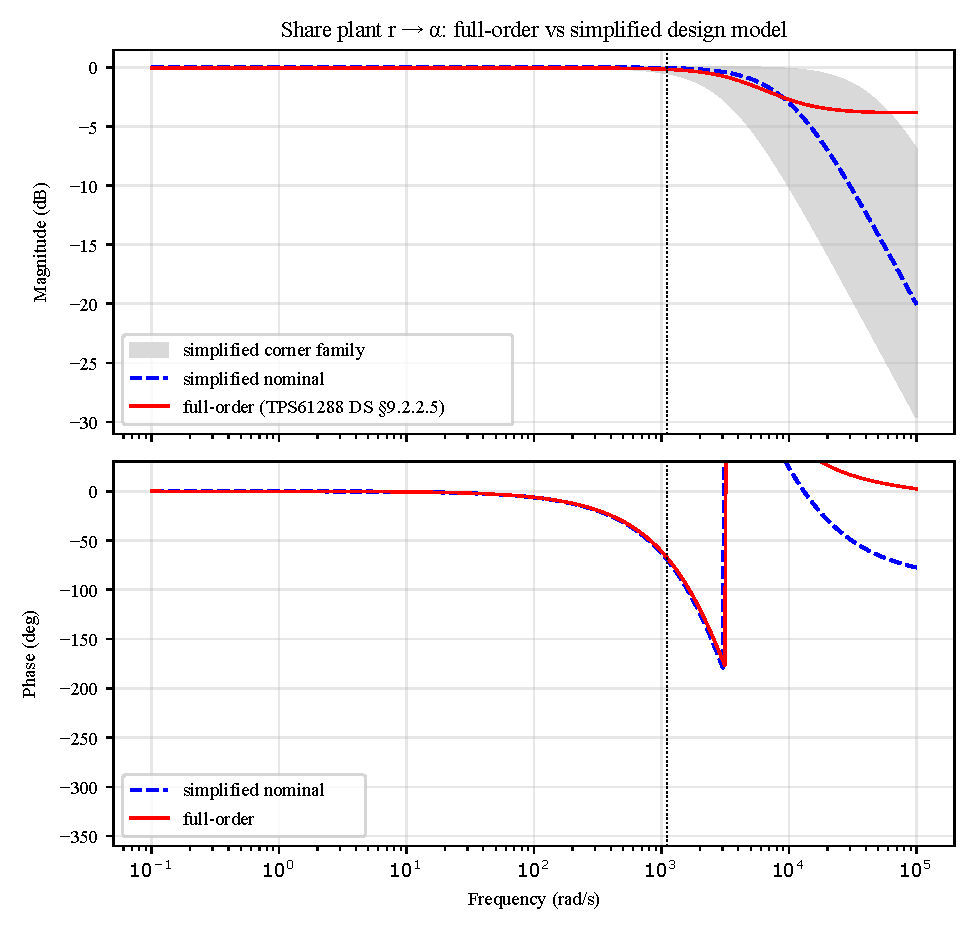
\includegraphics[width=\textwidth]{Figures/fullorder_bode_overlay.pdf}
% source: controller_design/figures/fullorder_bode_overlay.svg (data: fullorder_bode_overlay.csv)
\caption{Nominal open-loop frequency response of the 11-state full-order model overlaid on
the two-state-plus-delay design plant. The traces are visually indistinguishable through
the design band ($\omega\le\SI{1100}{\radian\per\second}$, max deviation \SI{3.86}{\percent})
and separate only beyond $\approx\SI{e4}{\radian\per\second}$, where the share-loop gain is
far below unity.}
\label{fig:fo-bode}
\end{figure}

\begin{figure}[H]
\centering
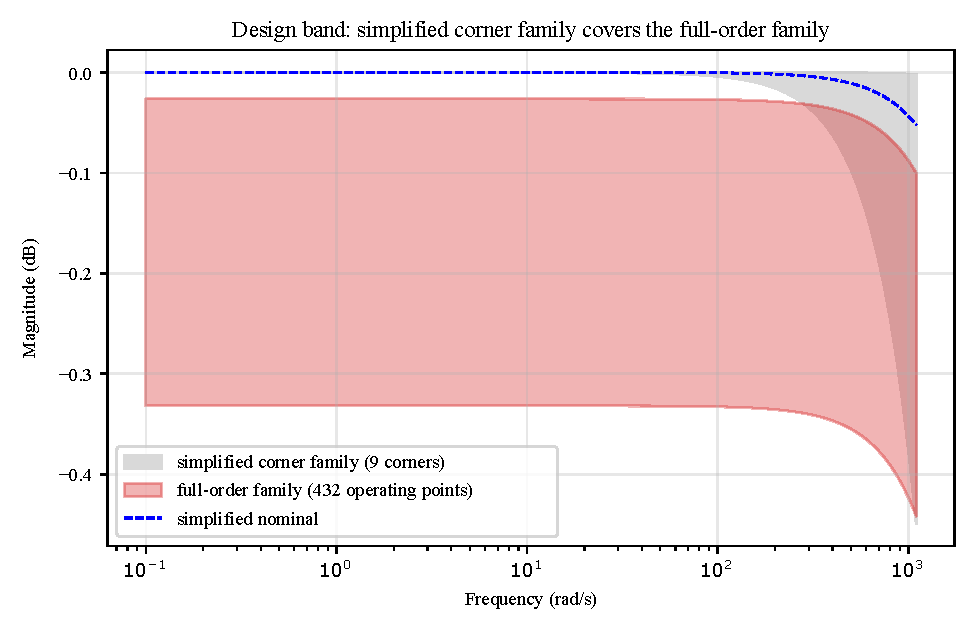
\includegraphics[width=\textwidth]{Figures/fullorder_envelope.pdf}
% source: controller_design/figures/fullorder_envelope.svg (data: fullorder_envelope.csv)
\caption{Envelope study: 432 full-order operating points against the simplified corner
family. The corner family bounds the full-order family with margin, which is the condition
for the synthesis uncertainty set to be valid.}
\label{fig:fo-envelope}
\end{figure}

\begin{figure}[H]
\centering
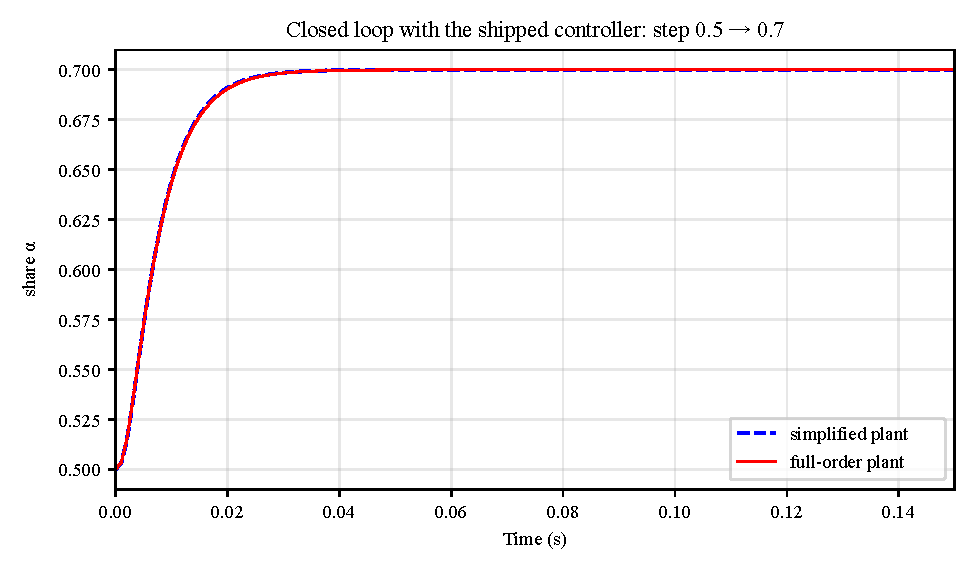
\includegraphics[width=\textwidth]{Figures/fullorder_step_overlay.pdf}
% source: controller_design/figures/fullorder_step_overlay.svg (data: fullorder_step_overlay.csv)
\caption{Closed-loop step response of the shipped controller on the full-order plant
overlaid on the design prediction. Maximum divergence is \num{0.0008} share.}
\label{fig:fo-step}
\end{figure}

\subsubsection{Independent toolchain cross-check}

Because the synthesis was performed in a purpose-written solver, the entire result was
re-derived in a commercial robust-control toolbox using the same weights, and the
\emph{shipped} coefficients --- parsed directly from the firmware header rather than
re-synthesised --- were re-run through the validation battery in the firmware-accurate
loop topology.

\begin{table}[H]
\caption{Independent toolbox cross-check of the shipped controller.}
\label{tab:matlab}
\begin{tabular}{lll}
\toprule
\textbf{Quantity} & \textbf{Independent toolbox} & \textbf{Design pipeline}\\
\midrule
$\gamma_{opt}$              & \num{0.6553}      & \num{0.6532} ($+\SI{0.3}{\percent}$)\\
$T_H(0)$                    & \num{0.99996378}  & \num{0.99996423}\\
$k_I$                       & \num{110.429}     & \num{111.930} ($+\SI{1.36}{\percent}$)\\
Crossover                   & \SI{109.4}{\radian\per\second} & \SI{109.9}{\radian\per\second}\\
Nominal $M_2$               & \num{0.796}       & \num{0.798}\\
Corner sweep                & 30/30 stable, worst $\|S\|_\infty=\num{1.768}$ & 60/60 stable, worst \num{1.867}\\
Step / DC gain              & \SI{25}{\milli\second} settle, DC gain \num{1.000000001} & \SI{22}{\milli\second} settle\\
\bottomrule
\end{tabular}
\end{table}
% All entries: MATLAB_validation.txt (VERDICT: PASS)

The two independent syntheses agree on $\gamma_{opt}$ to \SI{0.3}{\percent} and on the
nominal margins to within measurement resolution; the \SI{9.5}{\percent} frequency-response
deviation between the shipped and re-synthesised controllers is attributable to the
$21\to3$ order reduction plus two independent $\gamma$-iterations, and the meaningful
comparison --- closed-loop behaviour and corner stability --- agrees closely.
% MATLAB_validation.txt section B note

% ---------------------------------------------------------------------------
\subsection{Limitations}
\label{sec:share-limitations}

% NOTE (author): keep this subsection. Reviewers reward stated limitations, and every item
% here is genuinely open at time of writing.
Three qualifications bound the claims above. First, the plant timing parameters
($T_d$, $\tau_r$, $C_{bus}$, $\Delta V_0$ and the droop scale $k_d$) are pre-calibration
estimates; the corner sweep is the hedge, and the design is deliberately delay-tolerant
(\SI{11.7}{\milli\second} margin against \SI{2}{\milli\second} worst modelled). A bench
identification procedure --- open-loop $r$-sweep to fit $\Delta V_0$ and confirm unity
slope, plus a step test on the current-sense outputs to extract $\tau_r$ and the true
$T_d$ --- is defined, after which the coefficients are regenerated through the same
automated pipeline. Second, the plant gain is assumed positive over the operating set;
below about \SI{1}{\ampere} total current with worst-case mismatch the gain envelope
widens beyond the design set, so the supervisor must avoid commanding extreme shares at
near-zero load (the loop is in any case frozen as $I_{tot}\to 0$). Third, the analysis is
small-signal and continuous-conduction; pulse-frequency-mode operation at light load is
unmodelled, though even a \SI{1}{\milli\second} effective lag would cost only \ang{6.3} at
the share crossover, less than the phase already budgeted by the \SI{2}{\milli\second}
delay corner.

% ============================================================================
% PLANNING NOTES
% ============================================================================
% 1. FIGURE FILES. All figure sources exist as SVG in controller_design/figures/:
%      loopshapes_youla_h.svg, controller_bode.svg, timedomain_step_ramp.svg,
%      fullorder_bode_overlay.svg, fullorder_envelope.svg, fullorder_step_overlay.svg,
%      droop_signal_chain.svg, control_loop_model.svg
%    Each has a matching .csv of raw data. step_response_nominal.csv and
%    step_response_mismatch.csv have NO rendered figure yet -- Fig.~\ref{fig:step-openloop}
%    must be plotted from the CSVs (columns: t_s, r_cmd, alpha, v_bus) before submission.
%    MDPI wants PDF/EPS, not SVG: convert with inkscape/cairosvg into Figures/ and keep
%    the .pdf extension used in the \includegraphics calls above.
%
% 2. NUMERIC DRIFT WARNING. Several constants were retuned on 2026-07-11 (16 V bus
%    retune: R_D1 237k -> 215k, hence R_e,max 2.220 -> 2.014 Ohm, V_0 15.91 V,
%    k_d 0.33 -> 0.30 Ohm). This section uses the POST-retune values from
%    system_model.md. Older project notes still quote the pre-retune numbers -- do not
%    mix them. If bench calibration lands before submission, EVERY number in the
%    tables here changes: regenerate via synthesize_controller.py ->
%    tps61288_full_model.py -> droop_plant.m and re-extract from the generated
%    *_metrics.txt files rather than editing by hand.
%
% 3. CITATIONS TO ADD. The method reference (Tan, Yadav, Assadian, "A Practical
%    Youla Gain-Tuning Framework for H-infinity Controller Realization" — the
%    companion paper in papers/A_Practical_Youla_Gain_Tuning_Framework...) is cited in
%    prose but has no \cite key yet. Also needs: DGKF 1989 for the central-controller
%    formulation, a standard reference for balanced truncation, and datasheet citations
%    for the boost converter, current-sense amplifier and multiplying DAC. Part numbers
%    have been kept out of the prose deliberately -- decide whether the venue wants them
%    named or kept generic, and apply consistently.
%
% 4. SECTION LENGTH. As drafted this runs long for a single Energies section
%    (~8 figures, 6 tables). Candidate cuts if space is tight:
%      - fold the validation summary + MATLAB cross-check tables into one;
%      - move the full-order validation to an appendix, keeping only the
%        two headline numbers (<6% deviation, 432/432 stable) in the main text;
%      - drop Fig. fullorder_envelope, which is the least self-explanatory plot.
%    Do NOT cut the 26.9 vs 1.87 comparison or the T(0)=1 argument -- those are the
%    contribution.
%
% 5. UNRESOLVED / TO CONFIRM WITH BENCH DATA BEFORE THIS IS A PAPER RATHER THAN A PLAN:
%      - no experimental results at all yet; every number is model-derived. The paper
%        needs at minimum the CAL-1 static sweep (Delta V_0 fit) and CAL-2 step test
%        to claim validation rather than verification.
%      - the "legacy PI is near-unstable" claim is a simulation result at the corners,
%        not an observed instability. Word it carefully or obtain a bench demonstration.
%      - the firmware droop-mapping defect is currently fixed in code but
%        unverified on hardware; the CAL-1 sweep is what confirms the corrected mapping.
%
% 6. NOTATION CHECK. This section uses alpha for share, r for droop ratio, g for MDAC
%    gain, K for plant gain. Confirm none of these collide with other sections.
% ============================================================================
   % Plant modeling, H-inf/Youla synthesis, validation
% =====================================================================
% Section: Balancer Board Design and Droop Implementation Hardware
% Mock / planning-stage prose. Numeric values from CLAUDE.md, the IO CSV,
% and the BOM (rev 20260622); re-verify against the schematic PDF before
% publishing, especially anything flagged TODO(calibrate) in firmware.
% NOTE(orchestrator): bus nominal is quoted as 17.5 V below (rev-20260622
% design value). The 2026-07-08 plan / 2026-07-11 retune moved nominal to
% 16 V — reconcile with Section \ref{sec:droop} (which uses the 16 V-retune
% constants, V_0 = 15.91 V) before submission. One bus voltage, everywhere.
% =====================================================================

\section{Balancer Board Design and Droop Implementation Hardware}
\label{sec:board-design}

% NOTE(author): Open with the system-level framing: this is a purpose-built
% PCB (not an off-the-shelf BMS/charge-controller stack) because droop
% power sharing between two dissimilar sources needs an analog injection
% point that commercial boost modules don't expose. Argue that hardware
% co-design is a contribution in itself, not just a testbed.

\subsection{Overall Architecture}
\label{sec:board-architecture}

The balancer board (revision 20260622) implements a two-source,
bidirectional power-pathing architecture for a hybrid fuel-cell/battery
scale-model vehicle. Two independently regulated sources are combined onto
a common DC bus: a hydrogen fuel cell and a 2S lithium battery pack, each
boosted to the nominal bus voltage by an independent
TPS61288 synchronous boost converter (FC channel and BT channel). The two
boost outputs are not simply diode-ORed onto the bus; each is gated onto
the bus through a dedicated RT1987 ideal-diode power-path switch, so the
firmware -- not the analog hardware alone -- decides when each source is
allowed to contribute current.

% NOTE(author): Emphasize *why* ideal-diode switches instead of passive
% Schottky ORing: (1) negligible forward drop vs. a discrete diode at
% several amps, (2) true reverse-current blocking (no body-diode
% passthrough) so a disabled channel cannot be back-fed, which matters
% once regen braking is introduced, and (3) they are digitally
% controllable, which is the enabling feature for the sequencing state
% machine in Section~\ref{sec:power-pathing}.

Downstream of the bus, power flows through a further ideal-diode switch to
the VESC motor controller and the drive motor (\texttt{MOT\_PWR\_ENABLE}).
The motor is also the vehicle's regenerative braking source: during
deceleration the VESC can source current back onto the DC bus. This
current is intentionally \emph{not} routed back through the boost
converters -- doing so would require running a TPS61288 in reverse outside
its intended operating envelope and risks the back-feed hazard discussed
in Section~\ref{sec:power-pathing}. Instead, regenerated energy is routed
through a dedicated \texttt{REGEN\_ENABLE} path to the on-board battery
charger.

Battery charging is handled by two cooperating circuits with very
different bandwidths:

\begin{itemize}
  \item A \textbf{TL431/BSP170P shunt (chopper) clamp} is the
    \emph{fast}, board-local protection element. It is a fixed analog
    circuit (TL431 reference, BSP170P shunt MOSFET, dump resistor) with
    \emph{no firmware involvement} -- it exists to absorb the leading edge
    of a regen transient before any slower control loop can react, and to
    bound bus overvoltage independent of MCU state.
  \item A \textbf{Silvertel Ag105 MPPT module} is the \emph{secondary},
    slow harvester. It receives either fuel-cell bus power
    (\texttt{FC\_CHARGE\_ENABLE}) or regen power
    (\texttt{REGEN\_ENABLE}~+~\texttt{MOT\_PWR\_ENABLE}) and trickles it
    into the 2S pack under its own perturb-and-observe MPPT loop. Firmware
    controls it coarsely, through an active-low \texttt{MPPT\_DISABLE}
    GPIO and a two-register I\textsuperscript{2}C configuration write
    (voltage/current profile selection), not through a fast current-command
    interface.
\end{itemize}

% NOTE(author): This two-tier framing (fast passive clamp + slow active
% MPPT) is a good place to cite classic references on hybrid energy
% storage system power split (fast/slow filtering, e.g. supercapacitor
% + battery literature) even though the board doesn't literally have a
% supercapacitor -- the chopper is functionally the same kind of fast
% element.

A Teensy 4.1 (ARM Cortex-M7, \SI{600}{\mega\hertz}) is the sole controller
on the board. It executes the droop power-share control loop, the motor
current loop (talking to the VESC over UART), the sequencing state
machine for the ideal-diode switches, and the balancer/charger
supervisory logic, and exposes telemetry/command framing over UDP to a
Raspberry Pi bridge. A BQ29200 provides hardware-independent
overvoltage protection (OVP) on the individual battery cells; its
balance-enable pin is hardwired inactive, and only its OVP disable
(\texttt{CBAL\_DISABLE}) is under firmware control.

\subsection{Droop Implementation Hardware Chain}
\label{sec:droop-hardware}

% NOTE(author): This is the core novelty subsection -- spend the most
% care here. Argue explicitly that analog droop injection at the
% converter feedback node, commanded digitally by the MCU, is what lets
% a single control loop trade off "how much power-share authority do I
% have" against "how fast can I move it" without touching the boost
% converter's own fast voltage loop compensation.
% NOTE(orchestrator): the derivation/values live in Section \ref{sec:droop};
% keep this subsection qualitative (board-resource framing) to avoid
% duplication.

Each boost channel implements current-mode droop by perturbing its own
voltage-feedback divider in proportion to measured output current, so
that as a channel's current rises, its regulated bus voltage target sags
slightly -- the classical mechanism by which multiple sources sharing one
bus settle to a current split without a fast communication link between
them. On this board, the droop \emph{coefficient} is not fixed in
resistor value; it is a \emph{digitally commandable gain}, which is the
key hardware enabler for a closed-loop, MCU-mediated power-share
controller rather than a purely passive droop network. The signal chain
per channel is:

\begin{enumerate}
  \item \textbf{Current sense -- INA253A1IPWR.} A bidirectional,
    integrated-shunt current-sense amplifier sits at each boost channel's
    output, converting channel current to a ground-referenced analog
    voltage. The board specified the A3 variant (\SI{0.4}{\volt\per\ampere})
    but the A1 variant (\SI{0.1}{\volt\per\ampere}) was fitted by
    procurement error; firmware compensates with the corrected gain
    ($K_\text{sns} = \SI{0.1}{\volt\per\ampere}$).
  \item \textbf{Buffer/scale -- OPA197.} A rail-to-rail op-amp buffers and
    scales the sense voltage before it is (a) read back by the Teensy ADC
    for telemetry and share-error computation, and (b) used as the
    injection driver downstream of the MDAC.
  \item \textbf{Digitally-controlled attenuation -- AD5443 multiplying
    DAC.} A 12-bit MDAC (SPI, one per channel, independent chip-selects
    \texttt{CS\_MDAC\_FC} / \texttt{CS\_MDAC\_BT}) sits in the injection
    path and acts as a firmware-programmable attenuation
    element. This is what turns "droop coefficient" from a soldered
    resistor value into a run-time variable the power-share controller
    can command directly.
  \item \textbf{Feedback injection network.} The MDAC output is summed
    into each boost converter's own voltage-feedback divider through a
    dedicated injection resistor, so the converter's regulation setpoint
    is pulled down in proportion to (measured current) $\times$ (MDAC
    code), closing the droop loop at the analog level while the MCU sets
    only the gain.
\end{enumerate}

% NOTE(author): This is a good spot to state the board-level resource
% cost of droop as a design requirement, to motivate why this couldn't be
% bolted onto an off-the-shelf boost eval board: it needs (a) an isolated
% current-sense tap at each converter's output *before* the ideal-diode
% switch (so sensed current reflects only that channel's own contribution,
% not bus-shared current), (b) two independent SPI chip-selects plus a
% shared SPI bus (MOSI/MISO/SCK) reserved on the MCU, (c) two ADC channels
% per source (voltage division check + current sense) reserved out of the
% Teensy 4.1's analog pins, and (d) op-amp output headroom -- note that the
% OPA197 on this board is bodged to run from the 5 V rail rather than
% 3.3 V, which the droop-code-to-voltage mapping must account for.

Because the injection network taps into the converter's own compensated
feedback loop, the achievable droop range is bounded by the converter's
loop dynamics, not just by the MDAC's 12-bit resolution -- this is the
link between the board-level hardware described here and the plant model
used in the controller synthesis (Section~\ref{sec:robust}). The MCU-side
resource cost of this scheme is deliberately modest: one shared SPI bus,
two chip selects, two ADC channels per source for sense readback, and no
dedicated timer/PWM hardware -- the droop actuation is fully absorbed by
the analog injection network, leaving the MCU free to run the share
controller as a periodic software loop rather than a hardware peripheral.

\subsection{Power-Pathing: Ideal-Diode Switches and Sequencing}
\label{sec:power-pathing}

% NOTE(author): This subsection should read as a safety-case argument,
% not just a feature list -- the reviewer should come away understanding
% that the switch topology exists *because* naive "always-on" boost
% paralleling is unsafe with a bidirectional (regen) load, and that the
% sequencing rules are a direct, derivable consequence of that hazard,
% not arbitrary firmware policy.

Six RT1987 ideal-diode power-path switches, each independently controlled
by a Teensy GPIO, gate every power path on the board:

\begin{center}
\begin{tabular}{ll}
\texttt{FC\_BUS\_ENABLE} & FC boost $\rightarrow$ bus \\
\texttt{BT\_BUS\_ENABLE} & BT boost $\rightarrow$ bus \\
\texttt{MOT\_PWR\_ENABLE} & bus $\rightarrow$ VESC/motor node \\
\texttt{REGEN\_ENABLE} & regen node $\rightarrow$ charger \\
\texttt{FC\_CHARGE\_ENABLE} & bus (FC) $\rightarrow$ charger \\
\texttt{BT\_SEQUENCE\_ENABLE} & battery pack sequencing \\
\end{tabular}
\end{center}

This is a deliberate departure from a simpler "both boosts always
paralleled on the bus" design. Two hazards drive the sequencing
constraints:

\begin{itemize}
  \item \textbf{Back-feed / disabled-converter stress.} A converter that
    is disabled but still electrically connected to an energized bus can
    see reverse current or overshoot stress it was not designed for.
    Consequently, whenever the firmware brings a path up or down, the
    switch ordering is chosen so a regen or charge path is never left
    pointed at a converter that is not actively driving that node.
  \item \textbf{Hot-plug onto a discharged bulk capacitance.} Closing an
    ideal-diode switch onto a large discharged capacitor (the bus and,
    behind \texttt{MOT\_PWR\_ENABLE}, a \SI{470}{\micro\farad} node plus
    the VESC's own input capacitance) presents a near-short to the
    source side for the duration of the switch's soft-start ramp. If that
    ramp cannot supply the inrush within the switch's short-circuit
    protection window, the switch enters a burst-retry limit cycle, and
    the resulting repeated high-current transients have -- empirically,
    on this board -- destroyed boost converters (Section~\ref{sec:bringup}).
    This is why bus and motor-node bring-up is staged (switches first,
    allowed to settle, \emph{then} boosts; the motor node is pre-charged
    before \texttt{MOT\_PWR\_ENABLE} is closed) rather than done in one
    step.
\end{itemize}

The explicit rule set (mirrored in the firmware's power-path sequencing
guard) is: \texttt{BT\_SEQUENCE\_ENABLE} initializes off and is latched on
once during bring-up; \texttt{FC\_CHARGE\_ENABLE} requires
\texttt{BT\_BUS\_ENABLE} and \texttt{REGEN\_ENABLE} to both be low before
it is asserted (charger input path and regen path are mutually
exclusive); and \texttt{MOT\_PWR\_ENABLE} is only asserted onto a
pre-charged, sufficiently energized bus.

As a defense-in-depth measure independent of firmware correctness, every
enable net carries a \SI{10}{\kilo\ohm} pull-down to ground, so that
during MCU reset or any high-impedance boot window, every switch defaults
open (off) rather than floating into an undefined, possibly-closed state.

% NOTE(author): Good place to reference the incident log
% (docs/boost-bringup-debug.md) qualitatively -- "bench bring-up
% experience confirmed this hazard is not merely theoretical" -- the
% condensed version is Section \ref{sec:bringup}.

\subsection{Major Components}
\label{sec:bom-table}

% NOTE(author): Trim/reorder rows to taste; this table is meant to be a
% quick-reference companion, not a full BOM reproduction.

\begin{table}[H]
\centering
\caption{Major active components on the balancer board (rev.\ 20260622)
and their role in the droop / power-pathing architecture.}
\label{tab:major-ics}
\begin{adjustwidth}{-\extralength}{0cm}
\centering
\begin{tabular}{lll}
\toprule
\textbf{Component} & \textbf{Part} & \textbf{Role} \\
\midrule
FC / BT boost regulator & TI TPS61288 & Per-source boost to the DC bus, hosts droop injection \\
Ideal-diode power-path switch ($\times$6) & Richtek RT1987 & Digitally gated, reverse-blocking power path \\
Current-sense amplifier & TI INA253A1IPWR & Per-channel forward-current sense ($K_\text{sns}=0.1$\,V/A) \\
Droop MDAC & Analog Devices AD5443 & 12-bit, SPI-programmable droop-injection gain \\
MDAC output buffer & TI OPA197 & Rail-to-rail output driving injection network \\
Battery charger / MPPT & Silvertel Ag105 & Secondary harvester, I$^2$C config + \texttt{MPPT\_DISABLE} GPIO \\
Fast regen clamp & TI TL431 + Infineon BSP170P & Passive, board-local overvoltage / regen shunt \\
Cell OVP & TI BQ29200 & 2S cell overvoltage protection, \texttt{CBAL\_DISABLE} controlled \\
MCU & NXP i.MX RT1062 (Teensy 4.1) & Droop, sequencing, motor-loop, and telemetry controller \\
Motor controller & VESC (external) & UART motor current control, regen source \\
\bottomrule
\end{tabular}
\end{adjustwidth}
\end{table}

\subsection{Figures}
\label{sec:board-figures}

% NOTE(author): All three figures below are placeholders. Each TODO
% specifies exactly what the figure must communicate so a figure drawn
% later (in draw.io / KiCad / a photo) can be dropped in without
% re-deriving intent from scratch.

\begin{figure}[H]
  \centering
  % TODO: Draw a system block diagram showing:
  %   - Two source blocks: "Fuel Cell" and "2S Battery Pack"
  %   - FC boost (TPS61288) and BT boost (TPS61288) blocks downstream of
  %     each source, each annotated with its droop injection loop
  %     (INA253 -> OPA197 -> AD5443 -> feedback divider, drawn as a small
  %     closed loop back into the boost block, NOT as a separate top-level
  %     block, to show it's a local analog loop the MCU only sets the gain
  %     for)
  %   - FC_BUS_ENABLE / BT_BUS_ENABLE ideal-diode switches between each
  %     boost and a single "DC Bus" node
  %   - MOT_PWR_ENABLE switch from DC Bus to a "VESC + Motor" block
  %   - A regen arrow from "VESC + Motor" back toward the bus/regen node,
  %     clearly distinguished (dashed or colored) from the forward power
  %     flow arrows
  %   - REGEN_ENABLE and FC_CHARGE_ENABLE switches both feeding into the
  %     "Ag105 MPPT Charger" block, with a note that they are mutually
  %     exclusive
  %   - TL431/BSP170P "Fast Chopper Clamp" block shown directly on the
  %     regen node, NOT gated by any switch, to visually distinguish it
  %     from the firmware-controlled slow path
  %   - BQ29200 block on the battery pack with CBAL_DISABLE line from MCU
  %   - Single "Teensy 4.1" MCU block with lines fanning out to every
  %     enable/sense signal, labeled with the Code Names from the IO map
  \fbox{\parbox[c][5cm][c]{0.9\linewidth}{\centering PLACEHOLDER --- system
  block diagram; see TODO comment in source for required content}}
  \caption{Block diagram of the balancer board power and control
    architecture. \emph{[Placeholder -- diagram to be produced from the
    schematic.]}}
  \label{fig:block-diagram}
\end{figure}

\begin{figure}[H]
  \centering
  % TODO: Draw a power-path topology diagram (distinct from the block
  % diagram above -- this one should look like a simplified schematic /
  % single-line power diagram, not a signal-flow block diagram) showing:
  %   - Every RT1987 ideal-diode switch drawn as its actual topology
  %     symbol (or a diode-with-a-gate-control glyph), not a generic box
  %   - The six enable signals labeled at their respective switches using
  %     the exact Code Names
  %   - The 470uF bulk capacitor drawn explicitly at the motor/regen node
  %     to visually justify the hot-plug/pre-charge discussion
  %   - Hazard call-outs: (1) "back-feed risk" arrow at any
  %     switch-disabled-converter junction, (2) "inrush / hot-plug risk"
  %     bracket over the motor-node capacitance
  %   - A small inset legend distinguishing: always-open-by-default paths,
  %     latch-on-once paths (BT_SEQUENCE_ENABLE), and mutually-exclusive
  %     path pairs (FC_CHARGE_ENABLE vs. REGEN_ENABLE/BT_BUS_ENABLE)
  \fbox{\parbox[c][5cm][c]{0.9\linewidth}{\centering PLACEHOLDER ---
  power-path topology diagram; see TODO comment in source}}
  \caption{Power-path topology showing the six RT1987 ideal-diode
    switches, their sequencing constraints, and the hazard points that
    motivate them. \emph{[Placeholder -- to be produced from the
    schematic.]}}
  \label{fig:power-path-topology}
\end{figure}

\begin{figure}[H]
  \centering
  % TODO: Insert an annotated photo of the assembled board (rev 20260622)
  % once bench bring-up is far enough along to have a clean, populated
  % board shot (not mid-bodge). Annotate with call-out labels for:
  %   - FC and BT boost regulator sections
  %   - The RT1987 switch cluster
  %   - The Ag105 charger module footprint
  %   - The TL431/BSP170P chopper components
  %   - The BQ29200 balancer
  %   - The MDAC/OPA197 droop injection section
  %   - The Teensy 4.1 header location
  % If any bodge components (BT/FC output caps, RC-BT resistor swap,
  % RD1 215k) are visible/relevant, annotate them and note in the caption
  % that the photo reflects the as-bodged, not as-designed, board.
  \fbox{\parbox[c][5cm][c]{0.9\linewidth}{\centering PLACEHOLDER ---
  annotated board photo; see TODO comment in source}}
  \caption{Assembled balancer board (rev.\ 20260622), annotated.
    \emph{[Placeholder -- photo pending final bench assembly.]}}
  \label{fig:board-photo}
\end{figure}

% =====================================================================
% PLANNING NOTES
%
% 1. Numeric provenance: bus voltage, K_sns (0.1 V/A, INA253A1 variant
%    mixup), and the six enable-pin names are taken verbatim from
%    CLAUDE.md / the IO CSV / the BOM as of rev 20260622. Several firmware
%    constants referenced implicitly here (LIMIT_V_BUS_MAX, divider
%    scale factors, AG105_SETTLE_MS, BUS_SETTLE_MS) are still
%    TODO(calibrate) in the firmware itself -- do NOT state specific
%    values for those in the paper body until bench calibration lands.
%
% 2. BUS VOLTAGE INCONSISTENCY: this draft's original prose said 17.5 V;
%    the 2026-07-11 retune moved nominal to ~16 V (V_0 = 15.91 V in
%    Sec. \ref{sec:droop}). The explicit voltage has been removed from the
%    prose here; pick one number project-wide before submission.
%
% 3. The "hardware bodge" history (BT compensator resistor swap, output-
%    cap bodges, corrected failure analysis) is NOT in this section's
%    prose — it lives in Section \ref{sec:bringup}.
%
% 4. Unit macros: this section uses siunitx (\SI) and booktabs — both are
%    loaded via the main file preamble additions; verify they don't clash
%    with mdpi.cls.
%
% 5. Cross-check the component table part numbers/roles against the full
%    BOM CSV before submission (draft was built from BOM rows 1-102).
% =====================================================================
        % Balancer board, droop hardware chain, power pathing
% ============================================================================
%  SECTION: Bring-Up Failures, Modeling-Driven Diagnosis, and Fixes
%  Status: MOCK PROSE / PLANNING DRAFT. Numbers are traceable to
%  docs/boost-bringup-debug.md and tools/inductance/ results, but several are
%  flagged UNCONFIRMED in the source log and must not be hardened into claims
%  before the owed bench measurements land.
% ============================================================================

\section{Bring-Up Failures, Modeling-Driven Diagnosis, and Fixes}
\label{sec:bringup}

% NOTE: framing paragraph. The reviewer's likely reaction to a "we broke five
% converters" section is "why is this in a control paper?" -- answer that in the
% first sentence, not the last. The thesis-level claim is that the droop
% architecture was never implicated, and that establishing that required a
% modeling campaign of the same character as the control synthesis itself.

The power-sharing controller developed in Section~\ref{sec:synthesis} was designed
against a small-signal plant that presumes a functioning pair of boost converters
delivering current into a common DC bus. Reaching that operating point on hardware
proved substantially harder than reaching it in simulation: five TPS61288 boost
stages were destroyed over a six-week bring-up campaign, none of them while the
droop loop was closed. This section reports that campaign because its outcome is
methodologically relevant rather than merely anecdotal. Two of the three root
causes were identified only after building quantitative models---a Gerber-derived
parasitic-inductance extraction and a soft-start charge-transfer timing model---and
both models resolved questions that no amount of additional bench iteration had
resolved in four prior attempts. We also report the hypotheses that were wrong,
and the evidence that superseded them, because the discarded hypotheses were each
individually plausible and are each individually the standard textbook answer.

% ------------------------------------------------------------------
\subsection{Chronology of the Converter Failures}
\label{sec:bringup:chronology}

% NOTE: keep this table close to the original log's Failure Datapoints table.
% The key rhetorical move is that the *variance* across deaths is what kills
% each hypothesis -- 120 mA and 5 A both fatal, battery and bench supply both
% fatal, original and reworked parts both fatal.

All five failures shared an identical post-mortem signature: the converter's input,
switch, and output nodes fused to ground ($V_\mathrm{BT}\!\rightarrow\!\mathrm{GND}$
or $V_\mathrm{FC}\!\rightarrow\!\mathrm{GND}$ short), consistent with destruction of
the synchronous-rectifier FET. Table~\ref{tab:deaths} summarizes the conditions.

\begin{table}[H]
\caption{Converter failure events during bring-up. Deaths 1--4 are battery-channel;
Death~5 is fuel-cell-channel.\label{tab:deaths}}
\begin{adjustwidth}{-\extralength}{0cm}
\centering
\begin{tabular}{clll}
\toprule
\textbf{\#} & \textbf{Source} & \textbf{Action} & \textbf{Outcome} \\
\midrule
1 & Two \SI{9}{\volt} batteries & Enable BT$\rightarrow$bus ideal-diode switch & BT boost destroyed (original, never-reworked part) \\
2 & Bench supply, \SI{120}{\milli\ampere} limit & Firmware bring-up: switches, then boosts & Supply collapsed into current limit; BT boost destroyed \\
3 & Bench supply, $\geq$\SI{5}{\ampere} & Manual bring-up command & \SIrange{5}{7}{\ampere} with collapsed rail; BT boost destroyed \\
4 & Bench supply, \SI{8.2}{\volt}/\SI{200}{\milli\ampere} & Known-good FC part transplanted to BT pad & Immediate current-limit peg; BT boost destroyed \\
5 & FC from stiff bench supply, VESC attached & Close motor-node switch at full bus & FC boost destroyed \\
\bottomrule
\end{tabular}
\end{adjustwidth}
\end{table}

% NOTE: this paragraph is the "honest scientific narrative" the section is
% supposed to deliver. Do not soften it in revision -- the superseded
% hypotheses are the most transferable content here.

Four hypotheses were advanced and subsequently rejected. \emph{(i) Capacitive
inrush.} The obvious explanation for a converter dying at the instant it is
connected to a bus is inrush into bulk capacitance. This was refuted
topologically: the \SI{470}{\micro\farad} bulk capacitor sits on the motor node
\emph{behind} a separate ideal-diode switch, not on the shared bus, and that
switch was open in every one of Deaths~1--4. The bus itself carries only the
\SIrange{30}{40}{\micro\farad} of ceramics distributed across the ideal-diode
controllers. \emph{(ii) Source collapse and restart cycling.} Because the logic
rail is derived from the battery input through a linear regulator, a soft source
sags under converter load, browns out the microcontroller, and provokes a
re-enable cycle---a genuine failure mode observed on the bench. It was rejected as
\emph{the} cause because Death~3 occurred from a stiff $\geq$\SI{5}{\ampere}
supply that never collapsed, and Death~2 occurred at \SI{120}{\milli\ampere},
where the deliverable input energy is orders of magnitude below the destruction
energy. \emph{(iii) Reverse conduction through the disabled converter.} An early
design note asserted that a disabled boost presents a body-diode path through
which regenerative energy back-feeds the synchronous rectifier. Reading the
RT1987 ideal-diode datasheet retired this: the part uses back-to-back integrated
FETs and provides full isolation when disabled. The claim survived in the design
documentation for several weeks after it was falsified, and propagated into
firmware sequencing comments---a documentation-hygiene failure worth reporting.
\emph{(iv) Compensation-network mismatch.} The battery channel's compensation
resistor differed from the fuel-cell channel's; matching them was the intervention
in Death~4, which still destroyed the part.

Death~4 is the decisive experiment. A converter that had been \emph{proven good}
regulating on the fuel-cell pad was transplanted to the battery pad, verified to
regulate standalone, and then destroyed on its first bus connection. Combined with
three non-destructive control experiments---driving the bus node directly from a
supply with the converter removed (clean, $\approx$\SI{0}{\ampere}); driving the
bus from the fuel-cell converter (clean); and OR-ing a live bus against a supply
through the battery-side ideal diode (clean)---the fault was localized to the
\emph{battery channel's physical copper}, with the schematic confirmed identical
part-for-part. That conclusion, however, was reached by elimination, and
elimination does not produce a mechanism. Producing one required the modeling
described next.

% ------------------------------------------------------------------
\subsection{Parasitic-Inductance Extraction from Fabrication Gerbers}
\label{sec:bringup:inductance}

% NOTE: this is the subsection most likely to interest an Energies reviewer,
% because it is a reusable method rather than a board-specific war story.
% Consider promoting it to its own top-level section if the paper runs long
% in the control chapters.

The surviving hypothesis was that the battery channel's output-capacitor
commutation loop---the ``hot loop'' carrying the discontinuous current pulse when
the synchronous rectifier commutates---enclosed enough area to ring the switch node
past the device's \SI{20}{\volt} absolute-maximum rating under bus-drive
$\mathrm{d}i/\mathrm{d}t$, with only \SIrange{0.5}{1.5}{\volt} of nominal headroom
available. Physical measurement on the assembled board found the battery channel's
output ceramics placed \SI{240}{mil} from the converter output pin against
\SI{40}{mil} on the fuel-cell channel. A placement ratio, however, is not an
inductance ratio: all power nets on this board are polygon pours, so conductor
\emph{length} is a poor proxy and an earlier trace-length-based estimate was later
withdrawn as an artifact of a parser that excluded the pours.

We therefore built a dedicated extraction tool
(\texttt{tools/inductance/}) that computes loop inductance directly from the
fabrication data, with no manual geometry re-entry:

\begin{enumerate}
\item \textbf{Gerber and Excellon parsing.} A self-contained RS-274X and drill
parser converts the manufacturing files into copper polygons and hole locations,
so the extracted geometry is the geometry that was actually fabricated.
\item \textbf{Net isolation by flood fill.} Gerbers carry no net names; the forward
net (a converter-output pour) and the return net (the ground pour on the opposite
layer) are selected by coordinate and flood-filled at a fine isolation pitch, then
resampled to a coarser meshing pitch. Plane-clearance slots are morphologically
bridged so the return plane remains a single connected body at every pitch, with a
severed-plane detector that flags meshing artifacts.
\item \textbf{PEEC solution.} The meshed forward and return conductors are emitted
as a uniform-mesh FastHenry deck at their true stackup separation, with an explicit
port and an explicit loop closure at the load, and solved for
$L(f) = \operatorname{Im}\{Z_\mathrm{port}(f)\}/2\pi f$ over DC to \SI{1}{\mega\hertz}.
\item \textbf{Independent bound.} A closed-form microstrip estimate is computed from
the same mesh as a sanity check on the numerical result.
\end{enumerate}

% NOTE: emphasize the sweep design -- it is not a cross product, and that is a
% defensible methodological choice worth one sentence in a journal paper.

Because a PEEC result is only as trustworthy as its discretization, the tool solves
two orthogonal sweeps rather than a cross product: a \emph{mesh-convergence} axis
(all mesh pitches at one designated frequency) and a \emph{frequency} axis (all
frequencies at the converged pitch), sharing the designated point. Solutions are
persisted per-point to an append-as-you-go store, making multi-hour runs
interruptible and idempotent.

The result is given in Table~\ref{tab:Lsweep}. At the converged mesh, the
battery-channel output loop extracts to \SI{3.48}{\nano\henry} at DC falling to
\SI{3.15}{\nano\henry} at \SI{1}{\mega\hertz} (skin effect), against
\SI{1.54}{\nano\henry} and \SI{1.46}{\nano\henry} for the fuel-cell channel---a
ratio of $2.2\times$ at \SI{1}{\mega\hertz}. The two channels' extracted loop
\emph{lengths} (\SI{9.69}{\milli\meter} versus \SI{4.74}{\milli\meter}) and
effective widths (\SI{5.91}{\milli\meter} versus \SI{12.47}{\milli\meter}) show the
asymmetry is both a longer and a narrower return path.

% TODO(verify): CLAUDE.md and the debug log quote "~2.7x"; the current
% freq_sweep store gives 2.16x @ 1 MHz / 2.26x @ DC. The 2.7 figure predates a
% change in the loop-closure definition (pre-2026-07-01 L numbers are stale).
% Decide ONE number for the paper, cite the store that produced it, and delete
% the other everywhere. Do not publish both.

\begin{table}[H]
\caption{Extracted output-loop inductance, converged mesh.\label{tab:Lsweep}}
\begin{adjustwidth}{-\extralength}{0cm}
\centering
\begin{tabular}{lccccc}
\toprule
\textbf{Channel} & \textbf{Mesh (mm)} & $L$ \textbf{(DC)} & $L$ \textbf{(\SI{1}{\mega\hertz})} & \textbf{Loop len.} & \textbf{Eff. width} \\
\midrule
Fuel cell & 0.3 & \SI{1.538}{\nano\henry} & \SI{1.456}{\nano\henry} & \SI{4.74}{\milli\meter} & \SI{12.47}{\milli\meter} \\
Battery   & 0.2 & \SI{3.480}{\nano\henry} & \SI{3.149}{\nano\henry} & \SI{9.69}{\milli\meter} & \SI{5.91}{\milli\meter} \\
\bottomrule
\end{tabular}
\end{adjustwidth}
\end{table}

% NOTE: the fix + validation. The single-variable framing is the strongest
% claim in this whole section; state the controls explicitly.

The indicated remedy is a board-level one---firmware cannot reduce a loop
inductance. Ceramic capacitors of \SI{10}{\micro\farad} and \SI{0.1}{\micro\farad}
were bodged directly at the battery converter's output pins, collapsing the
\SI{240}{mil} loop to approximately the fuel-cell channel's geometry. The
validation was deliberately single-variable: an otherwise exact repetition of the
Death~4 configuration, differing only in the added capacitors. Where every
unmodified attempt had destroyed a converter, the modified channel survived
\emph{four consecutive} bring-ups, regulating the bus normally
(Figures~\ref{fig:scope-vout}--\ref{fig:scope-sw}).

% NOTE: this caveat is load-bearing for honesty. Do not cut it in editing.
Two limitations qualify this result. First, all validation captures were taken at
$1\times$ probe bandwidth ($\approx$\SI{10}{\mega\hertz}, \SI{50}{MSa/s}); the
hypothesized \SIrange{100}{200}{\mega\hertz} hot-loop ring is invisible at that
bandwidth. \emph{Survival is the evidence, not the waveform}, and a high-bandwidth
switch-node margin measurement remains owed. Second, the extraction models one
user-selected loop at a time and is not a full-board three-dimensional solve; it
supports a comparative claim between two nominally identical channels far better
than it supports an absolute ring-amplitude prediction.

% ------------------------------------------------------------------
\subsection{Soft-Start and Protection Timing in the Ideal-Diode Path}
\label{sec:bringup:softstart}

% NOTE: this is the subsection to sell to a *control* audience. Frame it as two
% independently designed loops (a fixed-timing open-loop charge ramp and a
% closed-loop voltage regulator) coupled through a node neither one models.

The hot-loop fix held for the battery channel, but a fifth converter---this time
on the fuel-cell side, with good layout---was destroyed while closing the motor-node
switch onto an attached motor controller. This failure has a different character
and is, in our view, the more generalizable one, because it arises from the
\emph{interaction of two independently designed control loops} rather than from a
layout defect.

The bus-to-motor path is gated by an RT1987 ideal-diode controller whose inrush
behavior is set by an open-loop soft-start ramp: a fixed external capacitance
($C_\mathrm{SS}=\SI{5.6}{\nano\farad}$) sets a turn-on time of order
\SI{1.1}{\milli\second}, during which a start-up short-circuit protection (SCP)
foldback current limit is armed with a \SI{250}{\micro\second} continuous-clamp
timer and a \SI{64}{\milli\second} retry interval. The ramp time is a designed
constant; it does not adapt to the load it is charging. Downstream sits the motor
node---\SI{470}{\micro\farad} of bulk capacitance plus the motor controller's own
(unmeasured) input capacitance, a total measured near \SI{590}{\micro\farad} on the
bare board. The charge demand of that node over the fixed ramp,
$I \approx 0.8\,C\,V/t_\mathrm{ON}$, lands in the same amperes-class range as the
applicable foldback limit. The ideal diode's protection therefore engages or nearly
engages on connection, and each clamp-and-release cycle presents the upstream boost
converters with a large, abrupt load step followed by an equally abrupt load dump.

% NOTE: the control-theoretic reading. This is the sentence the section exists for.
Neither loop is misdesigned in isolation. The ideal diode's soft start is a
correct open-loop inrush limiter for a bounded load capacitance; the boost's
voltage loop is a correctly compensated regulator with a \SIrange{4}{19}{\kilo\hertz}
crossover. The hazard lives in their coupling: the load-dump transient at the end
of a clamp interval occurs on a timescale comparable to the boost's loop latency,
so the boost error amplifier is left wound up delivering current into a suddenly
unloaded output. The resulting overshoot is then \emph{peak-held} by the ideal
diode itself, which cannot sink current---the switch behaves as a peak detector on
the bus, and the rail parks above nominal until leakage discharges it.
Measured parks of \SIrange{0.65}{0.72}{\volt} (centre-to-centre) above the
regulation point were observed, sufficient to trip the firmware bus overvoltage
fault on roughly \SI{80}{\percent} of bring-up attempts once the bus nominal was
retuned downward. At the \SI{15}{\ampere}-class currents of a full-bus motor-node
connection, the same event scaled past the converter's absolute-maximum rating and
destroyed it---but only from a stiff source, since a battery source sags into
undervoltage lockout before lethal current flows. This source dependence
retroactively explains the otherwise puzzling pattern across all five failures.

% TODO(verify): the log flags the *specific* clamp/cut identification as
% UNCONFIRMED and partially superseded -- the deepest observed event is now
% believed to be a soft-start that COMPLETED (1.77 ms conduction, current
% tapering as delta-V goes to zero) rather than a timer cut, and a smaller
% earlier event violates charge conservation by 14-300x and may be a rectified
% ring artifact of the unipolar current sensor. Write this subsection so that
% the *architectural* claim (fixed-ramp open-loop soft start vs. closed-loop
% regulator, coupled through an unmodeled capacitive node) survives regardless
% of which micro-mechanism wins at the bench. Do NOT publish the micro-mechanism
% as settled.

Two remedies follow directly, and are complementary. The firmware remedy is
\emph{sequencing}: never close the motor-node switch at full bus voltage. The
bring-up now raises the motor-node switch together with the bus switches
\emph{before} the boost converters ramp, so the converters' own soft start charges
the entire downstream stack from a low initial voltage in one coordinated ramp; the
node is then kept energized through idle and run states, with the motor held
stopped by a zero current command rather than by removing power. A guard predicate
faults rather than permitting a hot connection if the bus and motor-node
measurements indicate the node is discharged. This trades away hardware motor
isolation in idle---a deliberate and documented posture change. The hardware remedy
is to size the ideal diode's soft-start capacitance to the load it actually
charges: increasing $C_\mathrm{SS}$ from \SI{5.6}{\nano\farad} to
\SI{100}{\nano\farad} extends the ramp to tens of milliseconds and reduces the
connect demand to a few hundred milliamperes, restoring roughly an order of
magnitude of margin. A subsequent datasheet reconciliation also revealed that the
firmware's inter-phase settle delay had been sized from the soft-start time while
omitting the controller's \SI{8}{\milli\second} turn-on \emph{delay}, so the
intended coordinated ramp was not in fact executing; the current recommendation is
to replace the fixed delay with an ADC-confirmed pre-charge gate and timeout rather
than any tuned constant.

% ------------------------------------------------------------------
\subsection{Relationship to the Droop Architecture}
\label{sec:bringup:droop-relevance}

% NOTE: reviewers WILL ask whether droop caused any of this. Answer per-issue,
% in a table, and concede the one place where droop has genuine collateral
% (R_C is load-bearing for the share plant).

It is important to state precisely which of these hazards the droop power-sharing
architecture created, and which it merely inherited. Table~\ref{tab:droop-relevance}
gives the attribution.

\begin{table}[H]
\caption{Attribution of each bring-up hazard to architecture-specific versus generic causes.\label{tab:droop-relevance}}
\begin{adjustwidth}{-\extralength}{0cm}
\centering
\begin{tabular}{p{4.2cm}lp{7.5cm}}
\toprule
\textbf{Hazard} & \textbf{Attribution} & \textbf{Basis} \\
\midrule
Output hot-loop overshoot (Deaths 1--4) & Generic & A single-channel boost driving any capacitive bus exhibits it. The droop injection network was inactive (DACs unwritten) in every failure; the asymmetry is fabrication layout, present before any control code ran. \\
Motor-node hot-plug load dump (Death 5) & Generic multi-converter & Arises from an ideal-diode soft-start versus a downstream capacitive node; identical in a single-source system with the same power-path switching. \\
Ideal-diode peak-hold overvoltage parking & Generic & A consequence of non-sinking sources behind unidirectional switches; independent of how current is shared between them. \\
Source-collapse restart cycling & Generic (bench) & An artifact of deriving logic power from a converter input rail on a soft supply. \\
Droop-injection gain mapping error & \textbf{Droop-specific} & A firmware mapping omitted the feedback-injection attenuation, saturating both DACs and presenting the share loop a zero-gain plant. Non-destructive, but it invalidated all share-loop bench data taken before it was found (Section~\ref{sec:droop:bug}). \\
Compensation-resistor lever & \textbf{Coupled} & The obvious mitigation for load-dump overshoot---raising the boost crossover---is constrained because the compensation resistor sets the response time constant of the share-loop plant model, so a unilateral change would invalidate the synthesized controller. \\
\bottomrule
\end{tabular}
\end{adjustwidth}
\end{table}

The summary judgement is that the destructive failures were \emph{multi-converter
power-path bring-up hazards}, not droop-control hazards: they occurred with the
sharing loop open, with the modulating DACs at their reset state, and on a
single-channel basis. The droop architecture's genuine contribution to the campaign
was a non-destructive but consequential one---a gain-mapping error that silently
opened the share loop---and a constraint on the remedy space, in that the
compensation network is shared between the local voltage loop and the outer sharing
plant and cannot be retuned for transient margin without re-synthesizing the
controller. That coupling is, we would argue, the transferable control-level lesson:
in a droop-shared converter pair, the per-converter compensation network is no longer
a purely local design variable.

% ------------------------------------------------------------------
\subsection{Figures}
\label{sec:bringup:figures}

% NOTE: all placeholders. Scope JPGs exist under references/scope_captures/ and
% need re-export at publication resolution with cursors legible; the two drawn
% figures do not exist yet.

\begin{figure}[H]
\centering
% \includegraphics[width=0.8\textwidth]{Figures/scope-vout-validation.pdf}
\fbox{\parbox[c][4cm][c]{0.8\textwidth}{\centering PLACEHOLDER --- source:
\texttt{references/scope\_captures/1-VOUT.jpg}}}
\caption{Battery-converter output during a validated bring-up with hot-loop
capacitors fitted: body-diode pre-charge, one aborted soft-start attempt with
automatic retry, then clean regulation. The retry is a benign source-sag
undervoltage event, and is the same class of event that destroyed converters
before the fix.\label{fig:scope-vout}}
\end{figure}

\begin{figure}[H]
\centering
% \includegraphics[width=0.8\textwidth]{Figures/scope-triple.pdf}
\fbox{\parbox[c][4cm][c]{0.8\textwidth}{\centering PLACEHOLDER --- source:
\texttt{references/scope\_captures/5-Vout yellow-Vmot blue-Ibat purple.jpg}}}
\caption{Three-channel capture through a bring-up: converter output, bus voltage,
and current-sense output. The wide current hump is the downstream node charging
through a soft start that completes; the subsequent output park is the peak-held
overshoot.\label{fig:scope-triple}}
% TODO: cursor values in the raw capture are readable only at full resolution;
% re-export and annotate. Confirm the axis scaling caption (5 V/div, 5 A/div,
% 2 ms/div) against the instrument, not the log.
\end{figure}

\begin{figure}[H]
\centering
% \includegraphics[width=0.7\textwidth]{Figures/scope-sw-zoom.pdf}
\fbox{\parbox[c][3.5cm][c]{0.7\textwidth}{\centering PLACEHOLDER --- source:
\texttt{references/scope\_captures/3-SW.jpg}, \texttt{4-SW zoomed in.jpg}}}
\caption{Switch-node envelope during soft start. The initial discrete pulses are
normal pulse-frequency-modulation skipping, not instability. Note the bandwidth
limitation discussed in Section~\ref{sec:bringup:inductance}.\label{fig:scope-sw}}
\end{figure}

\begin{figure}[H]
\centering
% \includegraphics[width=0.8\textwidth]{Figures/inductance-sweep.pdf}
\fbox{\parbox[c][5cm][c]{0.8\textwidth}{\centering PLACEHOLDER --- generate from
\texttt{tools/inductance} frequency-sweep store}}
\caption{Extracted loop inductance versus frequency for both converter output
loops, with the mesh-convergence axis inset and the closed-form microstrip bound
shown for reference.\label{fig:Lsweep}}
% TODO: two-panel figure. (a) L(f) DC-1 MHz, both channels. (b) L vs mesh pitch
% at the designated frequency, showing convergence. Overlay the analytic bound
% as a dashed line -- it sits well below the solved value (0.64 vs 1.54 nH FC;
% 2.37 vs 3.48 nH BT) and that gap needs one sentence of explanation in the
% caption, since a reviewer will otherwise read it as a validation failure.
\end{figure}

\begin{figure}[H]
\centering
% \includegraphics[width=\textwidth]{Figures/fault-tree.pdf}
\fbox{\parbox[c][6cm][c]{\textwidth}{\centering PLACEHOLDER --- to be drawn}}
\caption{Campaign timeline and fault tree. Upper band: chronological failure and
intervention events. Lower band: hypothesis tree, with each branch annotated by the
experiment that refuted or confirmed it.\label{fig:faulttree}}
% TODO: draw in TikZ so it stays vector and editable. Suggested structure --
% root "converter destroyed on bus connect"; first-level branches: part defect,
% supply/source, bus path fault, firmware sequencing, channel layout; each leaf
% carrying its refuting experiment. Mark the surviving branch and the point at
% which Death 5 forced a second, independent root cause to be opened.
\end{figure}


% ============================================================================
% PLANNING NOTES
% ============================================================================
%
% PURPOSE OF THIS SECTION IN THE PAPER
% - Serves the "systems modeling" half of the thesis claim. The control chapters
%   show a model-based synthesis; this chapter shows model-based *diagnosis*.
%   Both leaned on building a quantitative model when iteration had stalled.
% - Secondary purpose: pre-empt the reviewer question "did your droop scheme
%   destroy your hardware?" The attribution table answers it explicitly and
%   concedes the one real coupling (compensation network shared between local
%   and sharing loops).
%
% OPEN ITEMS BEFORE THIS SECTION CAN BE SUBMITTED
% 1. INDUCTANCE RATIO DISCREPANCY. Project docs quote ~2.7x; the current results
%    store gives 2.16x @ 1 MHz. The discrepancy is a loop-closure definition
%    change (pre-2026-07-01 numbers are stale per project memory). Re-run the
%    sweep with the current closure on both configs, pick one number, and purge
%    the other from the paper, CLAUDE.md, and the debug log simultaneously.
% 2. ANALYTIC-BOUND GAP. The closed-form bound is ~2.4x below the solved value on
%    both channels. Consistent bias, so it does not threaten the comparative
%    claim, but a reviewer will ask. Either explain (bound neglects return-path
%    spreading / via inductance) or drop the bound from the figure entirely.
% 3. HIGH-BANDWIDTH RING MEASUREMENT IS STILL OWED. The entire hot-loop mechanism
%    rests on an inferred 100-200 MHz ring that has never been observed -- every
%    capture to date is ~10 MHz bandwidth. Until a 10x probe with a ground spring
%    captures the switch node at a controlled load step, the mechanism is
%    "consistent with all evidence", not "measured". Language throughout this
%    section must reflect that. Currently it does; keep it that way.
% 4. DEATH-5 MICRO-MECHANISM IS IN FLUX. The debug log has superseded its own
%    SCP-cut interpretation once already (a capture showed the soft start
%    completing rather than being cut). The architectural framing used here is
%    robust to that, but check the log's current state immediately before
%    submission and re-verify every number quoted in that subsection.
% 5. VESC INPUT CAPACITANCE IS UNMEASURED anywhere in the project. It appears in
%    the C_SS sizing argument as an unbounded term. Measure it, or drop the
%    quantitative margin claim to a qualitative one.
% 6. Deaths 1-4 count as "four battery-side boosts" in the summary doc but the
%    combined narrative with Death 5 makes five total. Make sure the abstract and
%    intro use the same count.
%
% STRUCTURAL DECISIONS TO REVISIT
% - The extraction-tool subsection may deserve promotion to its own methods
%   section or even a standalone short paper -- it is a reusable Gerber-to-PEEC
%   pipeline and is the most novel artifact here. Decide after the control
%   chapters are drafted and total length is known.
% - Consider moving the deaths table to an appendix and keeping only the
%   narrative, if Energies page pressure bites. The fault tree figure can carry
%   the chronology.
% - Tone check: the failure narrative is deliberately unflattering. That is the
%   point (superseded-hypothesis reporting is the contribution), but the
%   introduction to the chapter must frame it as method, not confession, or a
%   reviewer will read it as inexperience.
%
% CITATIONS TO ADD
% - TPS61288 datasheet (abs-max, OVP thresholds, compensation guidance §9.2.2.5)
% - RT1987 datasheet (tD_ON, soft-start timing, SCP foldback)
% - INA253 datasheet (unipolar sensing -- relevant to the half-rectified ring
%   caveat if that caveat survives into the final draft)
% - FastHenry / FastFieldSolvers, and a PEEC reference (Ruehli) for the method
% - A hot-loop layout reference (TI app notes on buck/boost layout) to
%   support the "Cout distance is the metric, not trace length" claim
% ============================================================================
   % Boost failures, inductance modeling tool, RT1987 soft-start
%=================================================================
% Section 6 — MIMO controller comparison (PLACEHOLDER — analysis not yet performed)
%=================================================================
\section{Toward a Combined MIMO Power--Drive Controller}
\label{sec:mimo}

% NOTE: This entire section is a placeholder. The analysis has NOT been performed.
% The purpose of including it in the plan is to (a) reserve the narrative slot,
% (b) define exactly what the comparison must contain so the future work is scoped,
% and (c) let reviewers of the outline see where the paper is headed.

The architecture presented so far treats the power-share loop (droop ratio $r$,
Section~\ref{sec:robust}) and the drive loop (motor current command from the velocity
controller) as decoupled SISO problems. In reality the two loops are coupled through the
bus: a drive transient changes the total load current, which both channels' droop
resistances convert into a share disturbance, while a share transient modulates the bus
voltage seen by the motor drive.
% NOTE: author to sharpen the physical coupling argument — the cross-coupling terms are
% visible in the full-order model (Section \ref{sec:robust}) as the bus-node interaction.

\subsection{Planned Comparison}
% TODO(analysis): none of the following exists yet. Planned scope:
\begin{itemize}
    \item Augment the share plant with the drive dynamics (VESC current loop approximated
          as a first-order lag + delay; motor/vehicle mechanical mode) to form a
          $2\times 2$ MIMO plant: inputs (droop ratio command, motor current command),
          outputs (measured share, wheel speed).
    \item Quantify the off-diagonal coupling (RGA / $\sigma$-plots) to establish whether
          the decentralized design is actually justified or merely convenient.
    \item Synthesize a MIMO $H_\infty$ controller on the same weight philosophy as
          Section~\ref{sec:robust} and compare against the decentralized pair on:
          worst-corner $\|S\|_\infty$, drive-transient share excursion, and regen-event
          bus excursion.
    \item Assess implementation cost on the Teensy 4.1 (state count vs.\ the current
          three-biquad realization at 1~kHz).
\end{itemize}

% FIGURE PLACEHOLDER
\begin{figure}[H]
    \centering
    \fbox{\parbox{0.9\linewidth}{\centering\vspace{2cm} TODO(figure): $2\times2$ MIMO block
    diagram — droop/share loop and drive loop with cross-coupling paths highlighted
    \vspace{2cm}}}
    \caption{Planned MIMO structure combining the power-share and drive loops.
    \textit{(Placeholder --- analysis not yet performed.)}}
    \label{fig:mimo_block}
\end{figure}

% PLANNING NOTES
% - Be explicit in the submitted paper that this is future work / outlook, OR perform the
%   RGA + synthesis before submission and promote it to a results section. Decide based on
%   page budget and thesis timeline.
% - The full-order 11-state model already contains the bus coupling; extending it with the
%   VESC lag is the cheapest path to the MIMO plant.
% - The EMS on the Pi commands share ≈ 1.0 during FC-charge cruise — the MIMO analysis
%   should include that operating point since the share loop is near an authority limit.
        % PLACEHOLDER: combined power-balance + drive MIMO controller
%=================================================================
% Section 7 — Conclusions (mock-up)
%=================================================================
\section{Conclusions}
\label{sec:conclusions}

% NOTE: mock prose — author to rewrite. Claims must mirror the abstract exactly.
This paper demonstrated that controllable power sharing between heterogeneous DC sources
can be implemented entirely with off-the-shelf regulator ICs by electronically injecting a
commanded droop resistance into each converter's feedback node, and that the resulting
share loop --- despite wide converter tolerance bands and channel asymmetry --- can be made
robust by $H_\infty$/Youla synthesis against an uncertainty-corner plant family.
% NOTE: 3–4 concluding claims, each traceable to a results section:
% 1. Droop injection chain (INA253 → MDAC → FB) achieves commandable share span [0.15, 0.85]
%    with no custom power stage. (Sec. 2/4)
% 2. Robust synthesis: worst-corner ||S||inf 1.87 vs 26.9 for nominal PI; validated by an
%    independent full-order model. (Sec. 3)
% 3. Bring-up failures were generic multi-converter hazards (layout hot-loop, ideal-diode
%    soft-start interaction), not droop-architecture defects; the modeling-driven diagnosis
%    method is itself a contribution. (Sec. 5)
% 4. Future work: MIMO combination with the drive loop (Sec. 6), bench calibration and
%    closed-loop share-step validation on the vehicle.

% PLANNING NOTES
% - Keep conclusions free of any number not established in the body.
% - MDPI Energies typically wants a short "future work" paragraph — fold Sec. 6 pointer here.


% ---------------- Back matter ----------------
\vspace{6pt}

\authorcontributions{Conceptualization, methodology, hardware, software, validation, writing: R.T. % TODO
}

\funding{This research received no external funding. % TODO: confirm
}

\dataavailability{The controller synthesis toolchain, plant models, and firmware are available from the author. % TODO: decide on repository release (GitHub/Zenodo DOI) — Energies encourages open data.
}

\conflictsofinterest{The author declares no conflicts of interest.}

%=====================================
% References — mock list lives with Section 1's draft for now.
% TODO: migrate to a .bib file + \bibliography once the reference set stabilizes.
%=====================================
% ============================================================================
% References — mock list for the planning draft.
% TODO(author): migrate to a .bib file once the reference set stabilizes.
% Items marked % TODO(verify) exist (publisher record hit during research) but
% author list / volume must be confirmed against Crossref before submission.
% ============================================================================
\begin{thebibliography}{99}

\bibitem{dragicevic2016part1}
Dragi\v{c}evi\'{c}, T.; Lu, X.; Vasquez, J.C.; Guerrero, J.M.
DC Microgrids---Part I: A Review of Control Strategies and Stabilization Techniques.
\emph{IEEE Trans. Power Electron.} \textbf{2016}, \emph{31}, 4876--4891.
\url{https://doi.org/10.1109/TPEL.2015.2478859}

\bibitem{dragicevic2016part2}
Dragi\v{c}evi\'{c}, T.; Lu, X.; Vasquez, J.C.; Guerrero, J.M.
DC Microgrids---Part II: A Review of Power Architectures, Applications, and Standardization Issues.
\emph{IEEE Trans. Power Electron.} \textbf{2016}, \emph{31}, 3528--3549.
\url{https://doi.org/10.1109/TPEL.2015.2464277}

\bibitem{gao2018primary}
Gao, F.; Kang, R.; Cao, J.; Yang, T.
Primary and secondary control in DC microgrids: a review.
\emph{J. Mod. Power Syst. Clean Energy} \textbf{2019}, \emph{7}, 227--242.
\url{https://doi.org/10.1007/s40565-018-0466-5}

\bibitem{guerrero2011hierarchical}
Guerrero, J.M.; Vasquez, J.C.; Matas, J.; de Vicu\~{n}a, L.G.; Castilla, M.
Hierarchical Control of Droop-Controlled AC and DC Microgrids---A General Approach Toward Standardization.
\emph{IEEE Trans. Ind. Electron.} \textbf{2011}, \emph{58}, 158--172.
\url{https://doi.org/10.1109/TIE.2010.2066534}

\bibitem{anand2013distributed}
Anand, S.; Fernandes, B.G.; Guerrero, J.M.
Distributed Control to Ensure Proportional Load Sharing and Improve Voltage Regulation in Low-Voltage DC Microgrids.
\emph{IEEE Trans. Power Electron.} \textbf{2013}, \emph{28}, 1900--1913.
\url{https://doi.org/10.1109/TPEL.2012.2215055}

\bibitem{lu2014adaptive}
Lu, X.; Sun, K.; Guerrero, J.M.; Vasquez, J.C.; Huang, L.
State-of-Charge Balance Using Adaptive Droop Control for Distributed Energy Storage Systems in DC Microgrid Applications.
\emph{IEEE Trans. Ind. Electron.} \textbf{2014}, \emph{61}, 2804--2815.
\url{https://doi.org/10.1109/TIE.2013.2279374}

\bibitem{tah2016adaptive}
Tah, A.; Das, D.
An Enhanced Droop Control Method for Accurate Load Sharing and Voltage Improvement of Isolated and Interconnected DC Microgrids.
\emph{IEEE Trans. Sustain. Energy} \textbf{2016}, \emph{7}, 1194--1204.
\url{https://doi.org/10.1109/TSTE.2016.2535264}

\bibitem{nasirian2015cooperative}
Nasirian, V.; Moayedi, S.; Davoudi, A.; Lewis, F.L.
Distributed Cooperative Control of DC Microgrids.
\emph{IEEE Trans. Power Electron.} \textbf{2015}, \emph{30}, 2288--2303.
\url{https://doi.org/10.1109/TPEL.2014.2324579}

\bibitem{tucci2018plugandplay}
Tucci, M.; Riverso, S.; Ferrari-Trecate, G.
Line-Independent Plug-and-Play Controllers for Voltage Stabilization in DC Microgrids.
\emph{IEEE Trans. Control Syst. Technol.} \textbf{2018}, \emph{26}, 1115--1123.
\url{https://doi.org/10.1109/TCST.2017.2695167}

\bibitem{kumar2020distributed}
Kumar, R.; Pathak, M.K.
Distributed droop control of dc microgrid for improved voltage regulation and current sharing.
\emph{IET Renew. Power Gener.} \textbf{2020}, \emph{14}, 2499--2506.
\url{https://doi.org/10.1049/iet-rpg.2019.0983}

\bibitem{khorsandi2024adaptive}
Al-Tameemi, Z.H.A.; Lie, T.T.; Foo, G.; Blaabjerg, F.
Adaptive Control Approach for Accurate Current Sharing and Voltage Regulation in DC Microgrid Applications.
\emph{Energies} \textbf{2024}, \emph{17}, 284.
\url{https://doi.org/10.3390/en17020284}

\bibitem{luo1999classification}
Luo, S.; Ye, Z.; Lin, R.-L.; Lee, F.C.
A classification and evaluation of paralleling methods for power supply modules.
In \emph{Proceedings of the 30th Annual IEEE Power Electronics Specialists Conference (PESC'99)}, Charleston, SC, USA, 27 June--1 July 1999; pp. 901--908.
\url{https://doi.org/10.1109/PESC.1999.785616}

\bibitem{panov2008stability}
Panov, Y.; Jovanovi\'{c}, M.M.
Stability and Dynamic Performance of Current-Sharing Control for Paralleled Voltage Regulator Modules.
\emph{IEEE Trans. Power Electron.} \textbf{2002}, \emph{17}, 172--179.
\url{https://doi.org/10.1109/63.988828}

\bibitem{schonberger2006dbs}
Schonberger, J.; Duke, R.; Round, S.D.
DC-Bus Signaling: A Distributed Control Strategy for a Hybrid Renewable Nanogrid.
\emph{IEEE Trans. Ind. Electron.} \textbf{2006}, \emph{53}, 1453--1460.
\url{https://doi.org/10.1109/TIE.2006.882012}

\bibitem{panda2021dbs}
Panda, S.K.; Ghosh, S.; Roy, T.K.
A novel dc bus-signaling based power management strategy for dc microgrid.
\emph{Int. Trans. Electr. Energy Syst.} \textbf{2021}, \emph{31}, e12758.
\url{https://doi.org/10.1002/2050-7038.12758}

\bibitem{vermillion2011mpc}
Vahidi, A.; Stefanopoulou, A.; Peng, H.
Model Predictive Control for Power Management in Hybrid Fuel Cell Vehicles.
In \emph{Proceedings of the IEEE Vehicle Power and Propulsion Conference}, Chicago, IL, USA, 6--9 September 2011.
\url{https://doi.org/10.1109/VPPC.2011.5043130}
% TODO(verify): confirm author list/year against IEEE Xplore record before submission.

\bibitem{hu2021mpcreview}
Yang, D.; Sun, X.; Wang, L.; Li, S.
A quantitative analysis of model predictive control as energy management strategy for hybrid electric vehicles: A review.
\emph{Energy Rep.} \textbf{2021}, \emph{7}, 6733--6755.
\url{https://doi.org/10.1016/j.egyr.2021.09.119}
% TODO(verify): author list — confirm on ScienceDirect record S2352484721009252

\bibitem{zhou2022mpc}
Zhou, Y.; Ravey, A.; P\'{e}ra, M.-C.
Multi-mode predictive energy management for fuel cell hybrid electric vehicles using Markov driving pattern recognizer.
\emph{Appl. Energy} \textbf{2020}, \emph{258}, 114057.
\url{https://doi.org/10.1016/j.apenergy.2019.114057}

\bibitem{thounthong2007control}
Thounthong, P.; Ra\"{e}l, S.; Davat, B.
Control Strategy of Fuel Cell and Supercapacitors Association for a Distributed Generation System.
\emph{IEEE Trans. Ind. Electron.} \textbf{2007}, \emph{54}, 3225--3233.
\url{https://doi.org/10.1109/TIE.2007.896477}

\bibitem{garcia2016statemachine}
Torreglosa, J.P.; Garc\'{i}a, P.; Fern\'{a}ndez, L.M.; Jurado, F.
Predictive Control for the Energy Management of a Fuel-Cell--Battery--Supercapacitor Tramway.
\emph{IEEE Trans. Ind. Inform.} \textbf{2014}, \emph{10}, 276--285.
\url{https://doi.org/10.1109/TII.2013.2245140}

\bibitem{li2022dcbusregulation}
Chen, X.; Xu, S.; Wang, Y.; Liu, Y.
Energy Management Strategy for PEM Fuel Cell Hybrid Power System Considering DC Bus Voltage Regulation.
\emph{Electronics} \textbf{2022}, \emph{11}, 2722.
\url{https://doi.org/10.3390/electronics11172722}
% TODO(verify): author list — confirm on the MDPI article page

\bibitem{sedhom2019hinf}
Sedhom, B.E.; Hatata, A.Y.; El-Saadawi, M.M.; Abd-Raboh, E.H.
Robust adaptive H-infinity based controller for islanded microgrid supplying non-linear and unbalanced loads.
\emph{IET Smart Grid} \textbf{2019}, \emph{2}, 420--435.
\url{https://doi.org/10.1049/iet-stg.2019.0024}

\bibitem{hosseinzadeh2024robust}
Kumar, J.; Agarwal, A.; Agarwal, V.
Stabilization of constant power loads and dynamic current sharing in DC microgrid using robust control technique.
\emph{Electr. Power Syst. Res.} \textbf{2024}, \emph{230}, 110251.
\url{https://doi.org/10.1016/j.epsr.2024.110251}
% TODO(verify): author list/volume — confirm on ScienceDirect S0378779624001469

\bibitem{mirjafari2022robust}
Mirjafari, S.M.M.; Bathaee, S.M.T.
Robust stability analysis of a novel droop-based distributed control scheme for islanded operation of DC microgrids.
\emph{IET Renew. Power Gener.} \textbf{2022}, \emph{16}, 2939--2953.
\url{https://doi.org/10.1049/rpg2.12585}

\end{thebibliography}


\end{document}
